\section{隐射(隐函数)与逆射(反函数)定理}\label{sec:8.4}

记 $F(x,y)$ 为 $n+1$ 元函数，其中 $\boldsymbol{x}=(x_{1},x_{2},\cdots,x_{n})$。于是，方程
\[
  \{(x,y) \mid F(x,y) = 0\}
\]
确定了 $\mathbb{R}^{n+1}$ 中的一个点集。问: 当 $F$ 满足什么条件时，$F(x,y)=0$ 才能确定一个隐函数 $y=f(x)$，且这个隐函数是 $C^{k}$ 的?

\begin{theorem}[隐函数存在定理]\label{thm:8.4.1}
记 $U \subset \mathbb{R}^{n+1}$ 为开集，$F: U \to \mathbb{R}^{1}$ 为 $n+1$ 元函数。如果

(1$^\circ$) $F \in C^{k}(U,\mathbb{R}^{1})$，$1 \leqslant k \leqslant +\infty$;

(2$^\circ$) $F(x^{0},y^{0}) = 0$，其中 $x^{0} = (x_{1}^{0},x_{2}^{0},\cdots,x_{n}^{0}) \in \mathbb{R}^{n}$，$y^{0} \in \mathbb{R}$，$(x^{0},y^{0}) \in U$ (即方程 $F(x,y) = 0$ 有解 $(x^{0},y^{0})$);

(3$^\circ$) $F_{y}^{\prime}(x^{0},y^{0}) \neq 0$.

则存在含 $(x^{0},y^{0})$ 的开区间 $I \times J$ ($I$ 为 $x^{0}$ 在 $\mathbb{R}^{n}$ 中的一个开区间，$J$ 为 $\mathbb{R}^{1}$ 中含 $y^{0}$ 的一个开区间)，如图 8.4.1 所示，使得:

(1) $\forall x \in I$，方程 $F(x,y) = 0$ 在 $J$ 中惟一解 $y = f(x)$，$f: I \to J$ 为 $n$ 元函数 (称 $f$ 为隐函数——隐藏在方程 $F(x,f(x)) = 0$ 中，但未必有明显的表达式);

(2) $y^{0} = f(x^{0})$;

(3) $f \in C^{k}(I,\mathbb{R}^{1})$;

(4) 当 $x \in I$ 时，$\dfrac{\partial f}{\partial x_{i}} = \dfrac{\partial y}{\partial x_{i}} = -\dfrac{F_{x_{i}}^{\prime}(x,y)}{F_{y}^{\prime}(x,y)}$，$i = 1,2,\cdots,n$，其中 $y = f(x)$.
\end{theorem}

\begin{figure}[htbp]
\centering
\begin{tikzpicture}[x=0.80cm, y=0.80cm, >=latex, line cap=round, line join=round]
  % 坐标轴
  \draw[line width=0.9pt, ->] (0, 0) -- (5.55, 0) node[below=-1pt, inner sep=1pt] {\small $x$};
  \draw[line width=0.9pt, ->] (0, 0) -- (0, 4.30) node[left=-1pt, inner sep=1pt] {\small $y$};
  \node[below left=-1pt, inner sep=1pt] at (0, 0) {\small $O$};
  % 开集 U
  \draw[line width=0.9pt, dashed]
    (2.55, 2.30) ellipse (2.30 and 1.42);
  \node[inner sep=1pt] at (3.62, 3.52) {\small $U$};
  % 区域 I x J(阴影矩形)
  \fill[pattern=north east lines, pattern color=black!45] (1.72, 1.72) rectangle (4.02, 3.02);
  \draw[line width=0.8pt, dashed] (1.72, 1.72) rectangle (4.02, 3.02);
  % 内部网格(示意 n 维分割)
  \draw[line width=0.5pt, dashed] (2.30, 1.72) -- (2.30, 3.02);
  \draw[line width=0.5pt, dashed] (2.87, 1.72) -- (2.87, 3.02);
  \draw[line width=0.5pt, dashed] (1.72, 2.50) -- (4.02, 2.50);
  \draw[line width=0.5pt, dashed] (1.72, 2.24) -- (4.02, 2.24);
  % 曲线 F(x,y)=0
  \draw[line width=1.0pt]
    (1.62, 2.92) .. controls (2.20, 2.98) and (2.70, 2.72) .. (3.35, 2.46)
    .. controls (3.95, 2.22) and (4.35, 2.02) .. (4.32, 1.62)
    .. controls (4.28, 1.28) and (3.85, 1.32) .. (3.62, 1.10);
  \node[anchor=west, inner sep=1pt] at (4.30, 1.78) {\small $F(x,y) = 0$};
  % 点 (x^0, y^0)
  \fill (3.05, 2.80) circle (1.3pt);
  \node[anchor=south, inner sep=1.5pt] at (3.28, 2.86) {\small $(x^{0},y^{0})$};
  % y^0 水平虚线
  \draw[line width=0.6pt, dashed] (0, 2.80) -- (4.02, 2.80);
  \node[anchor=east, inner sep=1.5pt] at (1.68, 2.80) {\small $y^{0}$};
  % I 下方大括号
  \draw[decorate, decoration={brace, amplitude=4.5pt, mirror}] (1.72, 0) -- (4.02, 0);
  \node[below=5pt, inner sep=1pt] at (2.87, -0.05) {\small $I$};
  % x, x^0 标记
  \node[below=-1pt, inner sep=1pt] at (2.30, 0) {\small $x$};
  \node[below=-1pt, inner sep=1pt] at (3.05, 0) {\small $x^{0}$};
  % J 左侧大括号
  \draw[decorate, decoration={brace, amplitude=4.5pt}] (0, 1.72) -- (0, 3.02);
  \node[left=6pt, inner sep=1pt] at (-0.06, 2.37) {\small $J$};
\end{tikzpicture}
\caption{}\label{fig:8.4.1}
\end{figure}

\begin{proof}
(1) 由条件 (3$^\circ$)，不妨设 $F_{y}^{\prime}(x^{0},y^{0}) > 0$，根据条件 (1$^\circ$)，存在含 $(x^{0},y^{0})$ 的开区间 $I_{0} \times J \subset U$，$F_{y}^{\prime}\mid_{I_{0} \times J} > 0$。于是，$\forall x \in I_{0}$，$F(x,\cdot)$ 在 $J$ 上严格增加。设 $J = (c,d)$，则由 (2$^\circ$)，必有 $F(x^{0},c) < 0$，$F(x^{0},d) > 0$。再由 (1$^\circ$)，$F \in C^{k}(U,\mathbb{R}^{1})$，故 $F$ 连续。因此，存在含 $x^{0}$ 的开区间 $I \subset I_{0}$，当 $x \in I$ 时，$F(x,c) < 0$，$F(x,d) > 0$。所以，$\forall x \in I$，$\exists_{1} y \in (c,d)$，s.t.\ $y = f(x)$。且 $F(x,f(x)) = F(x,y) = 0$ (见图 8.4.1)。

(2) 由 (2$^\circ$) 得到 $y^{0} = f(x^{0})$.

为证 (3) 与 (4)，先证 $f$ 在 $I$ 上连续。

$\forall x^{1} \in I$，设 $y^{1} = f(x^{1})$，$(x^{1},y^{1}) \in I \times J$。因为 $F(x^{1},y^{1}) = 0$，$F_{y}^{\prime}(x^{1},y^{1}) > 0$，故 $(x^{1},y^{1})$ 与 $(x^{0},y^{0})$ 满足相同的条件。于是，由前面所证知，$\exists I_{1} \times J_{1} \subset I \times J$，s.t.\ $(x^{1},y^{1}) \in I_{1} \times J_{1}$，且当 $x \in I_{1}$ 时，$F(x,y) = 0$ 在 $J_{1}$ 中有惟一解 $y = g(x)$，且 $y^{1} = g(x^{1})$.

$\forall \varepsilon > 0$，可取 $J_{1} = (y^{1} - \varepsilon,y^{1} + \varepsilon)$。于是，当 $x \in I_{1}$ 时，
\[
  y^{1} - \varepsilon = g(x^{1}) - \varepsilon < g(x) < g(x^{1}) + \varepsilon = y^{1} + \varepsilon.
\]
然而，由惟一性知，在 $I_{1}$ 上，$g = f$。这就证明了 $f$ 在 $x^{1}$ 处连续。又因 $x^{1} \in I$ 是任取的，故 $f$ 在 $I$ 上连续。

设 $x \in I$，取 $\Delta x$ 充分小，使 $x + \Delta x \in I$。记 $y = f(x)$，$\Delta y = f(x + \Delta x) - f(x)$。因为 $f$ 连续，故当 $\Delta x \to 0$ 时，$\Delta y \to 0$。于是，由 $F \in C^{k}(U,\mathbb{R}^{1})$，$k \geqslant 1$ 及定理 8.2.4 与定理 8.2.7 得到
\begin{align*}
  0 = 0 - 0 &= F(\boldsymbol{x} + \Delta \boldsymbol{x},f(\boldsymbol{x} + \Delta \boldsymbol{x})) - F(\boldsymbol{x},f(\boldsymbol{x})) \\
  &= F(\boldsymbol{x} + \Delta \boldsymbol{x},y + \Delta y) - F(\boldsymbol{x},f(\boldsymbol{x})) \\
  &= \sum_{i=1}^{n} F_{x_{i}}^{\prime}(\boldsymbol{x},y) \Delta x_{i} + F_{y}^{\prime}(\boldsymbol{x},y) \Delta y + \sum_{i=1}^{n} \alpha_{i} \Delta x_{i} + \beta \Delta y,
\end{align*}
其中 $\lim\limits_{\Delta x \to 0} \alpha_{i} = 0$，$\lim\limits_{\Delta x \to 0} \beta = 0$。由此立即推得
\begin{align*}
  \frac{\partial f}{\partial x_{i}} &= \frac{\partial y}{\partial x_{i}} = \lim_{\Delta x_{i} \to 0} \frac{\Delta y}{\Delta x_{i}} = -\lim_{\Delta x_{i} \to 0} \frac{F_{x_{i}}^{\prime}(\boldsymbol{x},y) \Delta x_{i} + \alpha_{i} \Delta x_{i}}{\left(F_{y}^{\prime}(\boldsymbol{x},y) + \beta\right) \Delta x_{i}} \\
  &= -\lim_{\Delta x_{i} \to 0} \frac{F_{x_{i}}^{\prime}(\boldsymbol{x},y) + \alpha_{i}}{F_{y}^{\prime}(\boldsymbol{x},y) + \beta} = -\frac{F_{x_{i}}^{\prime}(\boldsymbol{x},y)}{F_{y}^{\prime}(\boldsymbol{x},y)}.
\end{align*}
因为 $F \in C^{k}(U,\mathbb{R}^{1})$，所以 $F_{x_{i}}^{\prime} \in C^{k-1}(U,\mathbb{R}^{1})$。于是 $\dfrac{\partial f}{\partial x_{i}} \in C^{k-1}(I,\mathbb{R}^{1})$，$f \in C^{k}(I,\mathbb{R}^{1})$。
\end{proof}

\begin{theorem}[隐射存在定理]\label{thm:8.4.2}
设 $U \subset \mathbb{R}^{n+m}$ 为开集，$\boldsymbol{F}: U \to \mathbb{R}^{m}$ 为映射。如果

(1$^\circ$) $\boldsymbol{F} \in C^{k}(U,\mathbb{R}^{m})$，$1 \leqslant k \leqslant +\infty$;

(2$^\circ$) $\boldsymbol{F}(x^{0},y^{0}) = \boldsymbol{0}$，其中 $\boldsymbol{x}^{0} = (x_{1}^{0},x_{2}^{0},\cdots,x_{n}^{0})$，$\boldsymbol{y}^{0} = (y_{1}^{0},y_{2}^{0},\cdots,y_{m}^{0})$，$(x^{0},y^{0}) \in U$ (即方程 $\boldsymbol{F}(x,y) = \boldsymbol{0}$ 有解 $(x^{0},y^{0})$);

(3$^\circ$) 行列式
\[
  \det\begin{pmatrix}
    \dfrac{\partial F_{1}}{\partial y_{1}} & \cdots & \dfrac{\partial F_{1}}{\partial y_{m}} \\
    \vdots & & \vdots \\
    \dfrac{\partial F_{m}}{\partial y_{1}} & \cdots & \dfrac{\partial F_{m}}{\partial y_{m}}
  \end{pmatrix}_{(x^{0},y^{0})} = \det \boldsymbol{J}_{y}\boldsymbol{F}(x^{0},y^{0}) \neq 0,
\]
则存在含 $(x^{0},y^{0})$ 的一个开区间 $I \times J \subset U \subset \mathbb{R}^{n+m}$，使得:

(1) $\forall x \in I$，方程组 $F(x,y) = 0$ 在 $J$ 中有惟一解 $y = f(x)$，$f: I \to J$ 为映射 (称 $f$ 为隐射——隐藏在方程 $F(x,f(x)) = 0$ 中);

(2) $y^{0} = f(x^{0})$;

(3) $f \in C^{k}(I,\mathbb{R}^{m})$;

(4) 当 $x \in I$ 时，
\begin{align*}
  \boldsymbol{J}\boldsymbol{f}(\boldsymbol{x}) &= -\left(\boldsymbol{J}_{\boldsymbol{y}}\boldsymbol{F}(\boldsymbol{x},\boldsymbol{y})\right)^{-1} \boldsymbol{J}_{x}\boldsymbol{F}(\boldsymbol{x},\boldsymbol{y}) \\
  &= -\begin{pmatrix}
    \dfrac{\partial F_{1}}{\partial y_{1}} & \cdots & \dfrac{\partial F_{1}}{\partial y_{m}} \\
    \vdots & & \vdots \\
    \dfrac{\partial F_{m}}{\partial y_{1}} & \cdots & \dfrac{\partial F_{m}}{\partial y_{m}}
  \end{pmatrix}^{-1}
  \begin{pmatrix}
    \dfrac{\partial F_{1}}{\partial x_{1}} & \cdots & \dfrac{\partial F_{1}}{\partial x_{n}} \\
    \vdots & & \vdots \\
    \dfrac{\partial F_{m}}{\partial x_{1}} & \cdots & \dfrac{\partial F_{m}}{\partial x_{n}}
  \end{pmatrix},
\end{align*}
其中 $y = f(x)$.
\end{theorem}

\begin{proof}[对 $m$ 应用归纳法]
当 $m = 1$ 时，就是定理 8.4.1。

假设定理对 $m - 1$ 时成立。则当 $m$ 时，由条件 (1$^\circ$) 与 (3$^\circ$)，存在 $(x^{0},y^{0})$ 的开邻域 $U_{0} \subset U$，在 $U_{0}$ 上，$\det \boldsymbol{J}_{y}\boldsymbol{F} \neq 0$ 处处成立。

再由条件 (3$^\circ$)，$\dfrac{\partial F_{i}}{\partial y_{j}}(x^{0},y^{0})$ 不全为零，为叙述方便，不妨设 $\dfrac{\partial F_{m}}{\partial y_{m}}(x^{0},y^{0}) \neq 0$。并改记
\[
  (x,y) = (x,y_{1},y_{2},\cdots,y_{m-1},y_{m}) = (x,u_{1},u_{2},\cdots,u_{m-1},y_{m}) = (x,u,y_{m}),
\]
相应有 $(x^{0},y^{0}) = (x^{0},u^{0},y_{m}^{0})$，即
\[
  \frac{\partial F_{m}}{\partial y_{m}}(\boldsymbol{x}^{0},\boldsymbol{u}^{0},y_{m}^{0}) = \frac{\partial F_{m}}{\partial y_{m}}(\boldsymbol{x}^{0},\boldsymbol{y}^{0}) \neq 0.
\]
再由条件 (1$^\circ$)，$F_{m} \in C^{k}(U,\mathbb{R}^{1})$，又由条件 (2$^\circ$)
\[
  F_{m}(\boldsymbol{x}^{0},\boldsymbol{u}^{0},y_{m}^{0}) = F_{m}(\boldsymbol{x}^{0},\boldsymbol{y}^{0}) = 0.
\]
所以，根据定理 8.4.1，存在 $(x^{0},u^{0},y_{m}^{0})$ 的开区间 $\widetilde{I} \times \widetilde{J}_{m-1} \times \widetilde{J}_{1} \subset U_{0}$，使得

(1) $\forall (x,u) \in \widetilde{I} \times \widetilde{J}_{m-1}$，方程 $F_{m}(x,u,y_{m}) = 0$ 在 $\widetilde{J}_{1}$ 中有惟一解 $y_{m} = \varphi(x,u)$，其中 $\varphi: \widetilde{I} \times \widetilde{J}_{m-1} \to \widetilde{J}_{1}$ 为 $n+m-1$ 元函数;

(2) $\varphi(x^{0},u^{0}) = y_{m}^{0}$;

(3) $\varphi \in C^{k}(\widetilde{I} \times \widetilde{J}_{m-1},\mathbb{R}^{1})$.

这就表明，从方程组 $F(x,y) = 0$ 的最后一个方程 $F_{m}(x,u,y_{m}) = 0$ 中解出了隐函数 $y_{m} = \varphi(x,u)$，代入前 $m-1$ 个方程有
\[
  \left\{\begin{aligned}
    {} & F_{1}(x,u,\varphi(x,u)) = 0, \\
    {} & \vdots \\
    {} & F_{m-1}(x,u,\varphi(x,u)) = 0,
  \end{aligned}\right.
\]
其中 $(x,u) \in \widetilde{I} \times \widetilde{J}_{m-1}$。

令 $G_{i}(x,u) = F_{i}(x,u,\varphi(x,u))$，$i = 1,2,\cdots,m-1$，$(x,u) \in \widetilde{I} \times \widetilde{J}_{m-1}$。现考察 $\boldsymbol{G} = (G_{1},G_{2},\cdots,G_{m-1}): \widetilde{I} \times \widetilde{J}_{m-1} \to \mathbb{R}^{m-1}$。由 $G_{i}(x,u)$ 的定义及 $\varphi(x,u) \in \boldsymbol{C}^{k}(\widetilde{I} \times \widetilde{J}_{m-1},\mathbb{R}^{1})$ 可知，$\boldsymbol{G}$ 满足:
\begin{align*}
  (\widetilde{1}^{\circ}) \quad & \boldsymbol{G} \in C^{k}(\widetilde{I} \times \widetilde{J}_{m-1},\mathbb{R}^{m-1}); \\
  (\widetilde{2}^{\circ}) \quad & \boldsymbol{G}(\boldsymbol{x}^{0},\boldsymbol{u}^{0}) = (G_{1}(\boldsymbol{x}^{0},\boldsymbol{u}^{0}),G_{2}(\boldsymbol{x}^{0},\boldsymbol{u}^{0}),\cdots,G_{m-1}(\boldsymbol{x}^{0},\boldsymbol{u}^{0})) \\
  &= (F_{1}(\boldsymbol{x}^{0},\boldsymbol{u}^{0},\varphi(\boldsymbol{x}^{0},\boldsymbol{u}^{0})),F_{2}(\boldsymbol{x}^{0},\boldsymbol{u}^{0},\varphi(\boldsymbol{x}^{0},\boldsymbol{u}^{0})),\cdots,F_{m-1}(\boldsymbol{x}^{0},\boldsymbol{u}^{0},\varphi(\boldsymbol{x}^{0},\boldsymbol{u}^{0}))) \\
  &= (F_{1}(\boldsymbol{x}^{0},\boldsymbol{u}^{0},y_{m}^{0}),F_{2}(\boldsymbol{x}^{0},\boldsymbol{u}^{0},y_{m}^{0}),\cdots,F_{m-1}(\boldsymbol{x}^{0},\boldsymbol{u}^{0},y_{m}^{0})) \\
  &= (F_{1}(\boldsymbol{x}^{0},\boldsymbol{y}^{0}),F_{2}(\boldsymbol{x}^{0},\boldsymbol{y}^{0}),\cdots,F_{m-1}(\boldsymbol{x}^{0},\boldsymbol{y}^{0})) = (\boldsymbol{0},\boldsymbol{0},\cdots,\boldsymbol{0}) = \boldsymbol{0}.
\end{align*}

(3$^\circ$) 令 $\psi(x,u) = (x,u,\varphi(x,u))$，$\psi: \widetilde{I} \times \widetilde{J}_{m-1} \to \mathbb{R}^{n+m}$ 为 $C^{k}$ 映射。于是，
\[
  \binom{\boldsymbol{G}(x,u)}{F_{m}(x,u,\varphi(x,u))} = \binom{\boldsymbol{G}(x,u)}{\boldsymbol{0}} = \boldsymbol{F} \circ \psi(x,u).
\]
对该复合映射求“导”得
\begin{align*}
  \binom{\boldsymbol{J}G(x,u)}{\boldsymbol{0}} &= \begin{pmatrix} \boldsymbol{J}_{x}G & \boldsymbol{J}_{u}G \\ \boldsymbol{0} & \boldsymbol{0} \end{pmatrix} = \boldsymbol{J}\boldsymbol{F}(\psi(x,u))\boldsymbol{J}\psi(x,u) \\
  &= \left(\boldsymbol{J}_{x}\boldsymbol{F},\boldsymbol{J}_{u}\boldsymbol{F},\boldsymbol{J}_{y_{m}}\boldsymbol{F}\right)_{\psi(x,u)}
  \begin{pmatrix}
    \boldsymbol{I}_{n} & \quad \boldsymbol{0} \\
    \boldsymbol{0} & \boldsymbol{I}_{m-1} \\
    & \boldsymbol{J}_{x}\varphi & \boldsymbol{J}_{u}\varphi
  \end{pmatrix},
\end{align*}
其中 $\boldsymbol{I}_{n},\boldsymbol{I}_{m-1}$ 分别为 $n$ 阶、$m-1$ 阶单位矩阵。因此,
\begin{equation}
  \begin{pmatrix} \boldsymbol{J}_{u}G \\ \boldsymbol{0} \end{pmatrix} = \boldsymbol{J}_{u}\boldsymbol{F}(\boldsymbol{\psi}(x,u)) + \boldsymbol{J}_{y_{m}}\boldsymbol{F}(\boldsymbol{\psi}(x,u))\boldsymbol{J}_{u}\boldsymbol{\varphi}(x,u).
  \label{eq:8.4.1}
\end{equation}
另一方面，由条件 (3$^\circ$)，有
\begin{align*}
  \det\left(\frac{\partial \boldsymbol{F}}{\partial y_{1}},\frac{\partial \boldsymbol{F}}{\partial y_{2}},\cdots,\frac{\partial \boldsymbol{F}}{\partial y_{m}}\right)_{(x^{0},y^{0})}
  &= \det\left(\frac{\partial \boldsymbol{F}}{\partial u_{1}},\cdots,\frac{\partial \boldsymbol{F}}{\partial u_{m-1}},\frac{\partial \boldsymbol{F}}{\partial y_{m}}\right)_{(x^{0},u^{0},y_{m}^{0})} \\
  &\reason{行列式性质} \det\Bigl(\frac{\partial \boldsymbol{F}}{\partial u_{1}} + \frac{\partial \boldsymbol{F}}{\partial y_{m}}\frac{\partial\varphi}{\partial u_{1}},\frac{\partial \boldsymbol{F}}{\partial u_{2}} + \frac{\partial \boldsymbol{F}}{\partial y_{m}}\frac{\partial\varphi}{\partial u_{2}},\cdots, \\
  &\hspace{6.5em}\frac{\partial \boldsymbol{F}}{\partial u_{m-1}} + \frac{\partial \boldsymbol{F}}{\partial y_{m}}\frac{\partial\varphi}{\partial u_{m-1}},\frac{\partial \boldsymbol{F}}{\partial y_{m}}\Bigr)_{(x^{0},u^{0},y_{m}^{0})} \\
  &= \det\left(\boldsymbol{J}_{u}\boldsymbol{F} + \boldsymbol{J}_{y_{m}}\boldsymbol{F}\boldsymbol{J}_{u}\varphi,\frac{\partial \boldsymbol{F}}{\partial y_{m}}\right)_{(x^{0},u^{0},y_{m}^{0})} \\
  &= \det\begin{pmatrix} \boldsymbol{J}_{u}\boldsymbol{G} & \dfrac{\partial F_{1}}{\partial y_{m}} \\ & \vdots \\ \boldsymbol{0} & \dfrac{\partial F_{m}}{\partial y_{m}} \end{pmatrix}_{(x^{0},u^{0},y_{m}^{0})} \\
  &= \frac{\partial F_{m}}{\partial y_{m}}(x^{0},y^{0}) \cdot \det \boldsymbol{J}_{u}\boldsymbol{G}(x^{0},u^{0}),
\end{align*}
故有 $\det \boldsymbol{J}_{u}G(x^{0},u^{0}) \neq 0$。

上述推导表明 $\boldsymbol{G}$ 在 $(x^{0},u^{0})$ 满足定理的条件 (1$^\circ$)，(2$^\circ$)，(3$^\circ$)。由归纳假设，方程组 $\boldsymbol{G}(x,u) = \boldsymbol{0}$ 在含 $(x^{0},u^{0})$ 的区间 $I \times J_{m-1} \subset \widetilde{I} \times \widetilde{J}_{m-1} \subset \widetilde{I} \times \widetilde{J}$ 内，有:

($\tilde{1}$) 当 $x \in I$ 时，方程组 $G(x,u) = 0$ 在 $J_{m-1}$ 中有惟一解 $u = g(x)$，其中 $g: I \to J_{m-1}$ 为映射;

($\tilde{2}$) $u^{0} = g(x^{0})$;

($\tilde{3}$) $\boldsymbol{g} \in C^{k}(I,J_{m-1})$.

令 $f(x) = \begin{pmatrix} g(x) \\ \varphi(x,g(x)) \end{pmatrix}$，$x \in I$，$J = J_{m-1} \times \widetilde{J}$。于是，$f: I \to J$ 为映射，且满足定理结论的 (1)～(4).

(1) 当 $x \in I$ 时，$(x,g(x)) \in I \times J_{m-1} \subset \widetilde{I} \times J_{m-1}$。由 ($\tilde{1}$)，有
\[
  F_{i}(\boldsymbol{x},f(\boldsymbol{x})) = F_{i}(\boldsymbol{x},\boldsymbol{g}(\boldsymbol{x})),\quad
  \varphi(\boldsymbol{x},\boldsymbol{g}(\boldsymbol{x})) = G_{i}(\boldsymbol{x},\boldsymbol{g}(\boldsymbol{x})) = 0,\quad i = 1,2,\cdots,m-1,
\]
\[
  F_{m}(\boldsymbol{x},f(\boldsymbol{x})) = F_{m}\bigl(\boldsymbol{x},\boldsymbol{g}(\boldsymbol{x}),\varphi(\boldsymbol{x},\boldsymbol{g}(\boldsymbol{x}))\bigr) = 0,
\]
且 $g$ 和 $\varphi$ 都是惟一的，故
\[
  \boldsymbol{y} = f(\boldsymbol{x}) = \binom{\boldsymbol{g}(\boldsymbol{x})}{\varphi(\boldsymbol{x},\boldsymbol{g}(\boldsymbol{x}))}
\]
为方程组 $\boldsymbol{F}(\boldsymbol{x},\boldsymbol{y}) = \boldsymbol{0}$ 在 $J$ 中的惟一解.

(2) $u^{0} = g(x^{0})$ 与 $f(x^{0}) = \begin{pmatrix} g(x^{0}) \\ \varphi(x^{0},g(x^{0})) \end{pmatrix} = \begin{pmatrix} u^{0} \\ y_{m}^{0} \end{pmatrix} = y^{0}$.

(3) 因为 $\boldsymbol{g} \in C^{k}(I,J_{m-1})$，$\varphi \in C^{k}(\widetilde{I} \times \widetilde{J}_{m-1},\mathbb{R}^{1})$，所以 $f = \begin{pmatrix} \boldsymbol{g} \\ \varphi \end{pmatrix} \in C^{k}(I,\mathbb{R}^{m})$.

(4) 当 $x \in I$ 时，$x \mapsto \begin{pmatrix} x \\ f(x) \end{pmatrix} \mapsto F(x,y)$，且 $\boldsymbol{F}(\boldsymbol{x},f(\boldsymbol{x})) \equiv \boldsymbol{0}$. 对此等式复合求导得
\begin{align*}
  \boldsymbol{0} &= \boldsymbol{J}\boldsymbol{F}(\boldsymbol{x},f(\boldsymbol{x}))\begin{pmatrix} \boldsymbol{I}_{n} \\ \boldsymbol{J}f(\boldsymbol{x}) \end{pmatrix} = \left(\boldsymbol{J}_{x}\boldsymbol{F}(\boldsymbol{x},f(\boldsymbol{x})),\boldsymbol{J}_{y}\boldsymbol{F}(\boldsymbol{x},f(\boldsymbol{x}))\right)\begin{pmatrix} \boldsymbol{I}_{n} \\ \boldsymbol{J}f(\boldsymbol{x}) \end{pmatrix} \\
  &= \boldsymbol{J}_{x}\boldsymbol{F}(\boldsymbol{x},f(\boldsymbol{x})) + \boldsymbol{J}_{y}\boldsymbol{F}(\boldsymbol{x},f(\boldsymbol{x}))\boldsymbol{J}f(\boldsymbol{x}).
\end{align*}
由条件 $\det \boldsymbol{J}_{y}\boldsymbol{F}(x,f(x)) \neq 0$，$(x,y) \in U_{0}$，故 $\boldsymbol{J}_{y}\boldsymbol{F}$ 可逆。于是,
\[
  \boldsymbol{J}f(x) = -\left(\boldsymbol{J}_{y}\boldsymbol{F}\bigl(x,f(x)\bigr)\right)^{-1}\boldsymbol{J}_{x}\boldsymbol{F}\bigl(x,f(x)\bigr).
\]
从上述可看出 $\boldsymbol{J}f \in C^{k-1}(I,\mathbb{R}^{mn})$，因而 $f \in C^{k}(I,\mathbb{R}^{m})$。
\end{proof}

\begin{remark}\label{rem:8.4.1}
在定理 8.4.2 中，由 $\boldsymbol{F}(\boldsymbol{x},f(\boldsymbol{x})) \equiv \boldsymbol{0}$ 得到
\[
  \boldsymbol{J}_{x}\boldsymbol{F}(x,f(x)) + \boldsymbol{J}_{y}\boldsymbol{F}(x,f(x))\boldsymbol{J}_{x}f \equiv \boldsymbol{0},
\]
\[
  \boldsymbol{J}_{x}f = -\left(\boldsymbol{J}_{y}\boldsymbol{F}(x,f(x))\right)^{-1}\boldsymbol{J}_{x}\boldsymbol{F}(x,f(x)).
\]
\end{remark}

为研究逆射(反函数)定理，先举两个简单的例子.

\begin{example}\label{ex:8.4.1}
设一元函数 $f: I \to \mathbb{R}^{1}$，$y = f(x)$ 在 $I$ 上连续，在 $\overset{\circ}{I}$ 内可导，其中 $I$ 为区间，且 $y' = f'(x) \neq 0$，$\forall x \in \overset{\circ}{I}$。由此可推出在 $\overset{\circ}{I}$ 上恒有 $f'(x) > 0$ 或恒有 $f'(x) < 0$ (反证) 假设 $\exists x_{1},x_{2} \in \overset{\circ}{I}$，s.t.\ $f'(x_{1}) < 0 < f'(x_{2})$，由 Darboux 导函数介值定理知，$\exists \xi \in \overset{\circ}{I}$，s.t.\ $f'(\xi) = 0$，这与 $f'(x) \neq 0$，$\forall x \in \overset{\circ}{I}$ 矛盾). 这表明 $f$ 在 $I$ 上严格增或严格减，从而 $y = f(x)$ 在 $I$ 上有反函数 $x = f^{-1}(y)$. 进而，有
\[
  x_{y}^{\prime} = \frac{\mathrm{d}x}{\mathrm{d}y} = \frac{1}{y_{x}^{\prime}} = \frac{1}{f'(x)} = \frac{1}{f'(f^{-1}(y))}.
\]
\end{example}

\begin{example}\label{ex:8.4.2}
设 $z = x + \mathrm{i}y$，$w = u + \mathrm{i}v$，$x,y,u,v \in \mathbb{R}$，考虑复变量 $z$ 的复值函数(简称复函数)，
\[
  u + \mathrm{i}v = w = e^{z} = e^{x + \mathrm{i}y} = e^{x}(\cos y + \mathrm{i}\sin y),
\]
即
\[
  T\colon \left\{\begin{aligned}
    u &= e^{x}\cos y, \\
    v &= e^{x}\sin y.
  \end{aligned}\right.
\]
它可视作平面 $\mathbb{R}^{2}$ 到自身的一个 $C^{\omega}$ 映射，其 Jacobi 行列式为
\[
  \frac{\partial(u,v)}{\partial(x,y)} = \det\begin{pmatrix} e^{x}\cos y & -e^{x}\sin y \\ e^{x}\sin y & e^{x}\cos y \end{pmatrix} = e^{2x}(\cos^{2}y + \sin^{2}y) = e^{2x},
\]
由于 $w' = \dfrac{\mathrm{d}w}{\mathrm{d}z} = (e^{z})' = e^{z}$，
\[
  \left\|\frac{\mathrm{d}w}{\mathrm{d}z}\right\| = \|e^{z}\| = \|e^{x}(\cos y + \mathrm{i}\sin y)\| = \sqrt{e^{2x}(\cos^{2}y + \sin^{2}y)} = e^{x},
\]
所以
\[
  \frac{\partial(u,v)}{\partial(x,y)} = \left\|\frac{\mathrm{d}w}{\mathrm{d}z}\right\|^{2} = e^{2x} > 0.
\]
值得注意的是，即使 Jacobi 行列式处处大于零，映射 $(x,y) \mapsto (e^{x}\cos y,e^{x}\sin y)$ $(z \mapsto w = e^{z})$ 也未必有逆映射。事实上，从 $T(x,y) = T(x,y + 2k\pi)$ 可知 $T$ 甚至不是单射，因而无逆射。

但是，从 $\mathbb{R}^{n}$ 中的开集到 $\mathbb{R}^{n}$ 的映射有下面定理.
\end{example}

\begin{theorem}[局部逆射定理]\label{thm:8.4.3}
设 $D \subset \mathbb{R}^{n}$ 为开集，$f: D \to \mathbb{R}^{n}$ 为映射。如果

(1$^\circ$) $f \in C^{k}(D,\mathbb{R}^{n})$，$1 \leqslant k \leqslant +\infty$;

(2$^\circ$) $f(x^{0}) = y^{0}$，$x^{0} \in D$，$y^{0} \in \mathbb{R}^{n}$;

(3$^\circ$) $\det \boldsymbol{J}f(x^{0}) \neq 0$.

则存在 $x^{0}$ 的开邻域 $U$ 与 $y^{0}$ 的开邻域 $V$，使得

(1) $f(U) = V$，且 $f$ 在 $U$ 上为单射;

(2) 记 $g$ 为 $f$ 在 $U$ 上的逆映射，$g \in C^{k}(V,U)$;

(3) 当 $y \in V$ 时，$\boldsymbol{J}g(y) = \left(\boldsymbol{J}f(x)\right)^{-1}$，其中 $x = g(y)$ $(y = f(x))$. 此时，$f: U \to V$ 为 $C^{k}$ 微分同胚。
\end{theorem}

\begin{proof}
令 $F(x,y) = f(x) - y$，$(x,y) \in D \times \mathbb{R}^{n}$，它为映射，且

(1$^\circ$) $\boldsymbol{F}: D \times \mathbb{R}^{n} \to \mathbb{R}^{n}$，$\boldsymbol{F} \in C^{k}(D \times \mathbb{R}^{n},\mathbb{R}^{n})$;

(2$^\circ$) $\boldsymbol{F}(x^{0},y^{0}) = f(x^{0}) - y^{0} = y^{0} - y^{0} = \boldsymbol{0}$;

(3$^\circ$) $\boldsymbol{J}_{x}\boldsymbol{F}(x^{0},y^{0}) = \boldsymbol{J}f(x^{0})$，故 $\det \boldsymbol{J}_{x}\boldsymbol{F}(x^{0},y^{0}) = \det \boldsymbol{J}f(x^{0}) \neq 0$.

根据定理 8.4.2(隐射存在定理)，存在含 $(x^{0},y^{0})$ 的开区间 $I \times J \subset D \times \mathbb{R}^{n}$ 使得 $\forall y \in J$，方程 $F(x,y) = 0$，即 $y = f(x)$ 在 $I$ 中有唯一解 $x = g(y)$，其中 $g \in C^{k}(J,I)$；$x^{0} = g(y^{0})$；且当 $y \in J$ 时，
\begin{align*}
  \boldsymbol{J}g(y) &= -\left(\boldsymbol{J}_{x}\boldsymbol{F}(x,y)\right)^{-1}\boldsymbol{J}_{y}\boldsymbol{F}(x,y) \\
  &= -\left(\boldsymbol{J}f(x)\right)^{-1}(-\boldsymbol{I}_{n}) = \left(\boldsymbol{J}f(x)\right)^{-1},
\end{align*}
其中 $x = g(y)$.

令 $V = J$，$U = g(J) = g(V)$，显见 $V = f(U)$，$f: U \to V$ 与 $g: V \to U$ 互为逆映射。余下只需证明 $U$ 为开集。事实上，由于 $V = J$ 为开集与 $f$ 连续可知，$f^{-1}(V)$ 为开集。又因 $I$ 为开集，故 $U = g(V) = I \cap f^{-1}(V)$ 也为开集。
\end{proof}

\noindent 特别应注意的是，定理 8.4.3 只具有局部性质，只在点 $f(x^{0})$ 的近旁才存在着逆映射。即使当 $\det \boldsymbol{J}f$ 在 $D$ 上处处不等于零，也只能断言在 $f(D)$ 中的每一个点的一个局部范围内存在着逆映射，而不是在大范围内成为 $f$ 在 $f(D)$ 上的逆映射。而例 8.4.2 正是说明这个问题的一个典型反例。

如果再加强条件，就有如下的整体逆射定理.

\begin{theorem}[整体逆射定理]\label{thm:8.4.4}
设 $U \subset \mathbb{R}^{n}$ 为开集，$f: U \to \mathbb{R}^{n}$ 为映射。如果

(1) $f \in C^{k}(U,\mathbb{R}^{n})$，$1 \leqslant k \leqslant +\infty$;

(2) $\forall x \in U$，$\det \boldsymbol{J}f(x) \neq 0$;

则 $V = f(U)$ 为开集。又如果

(3) $f$ 在 $U$ 上为单射.

则 $f$ 有逆映射 $f^{-1}: V \to U$，即 $x = f^{-1}(y)$，$y = f(x)$。此外，$f^{-1} \in C^{k}(V,U)$，且
\[
  \boldsymbol{J}f^{-1}(y) = \left(\boldsymbol{J}f(x)\right)^{-1},
\]
其中 $x = f^{-1}(y)$.
\end{theorem}

\begin{proof}
$\forall y^{0} \in V$，$\exists x^{0} \in U$，s.t.\ $y^{0} = f(x^{0})$. 由定理 8.4.3，存在 $x^{0}$ 的开邻域 $U_{0}$ 与 $y^{0}$ 的开邻域 $V_{0}$ 满足 $V_{0} = f(U_{0})$. 因此，$V_{0} = f(U_{0}) \subset f(U) = V$，这表明 $y^{0}$ 为 $V$ 的一个内点. 由于 $y^{0}$ 是任取的，故 $V$ 全由内点组成，所以 $V = f(U)$ 为开集.

由于 $f$ 为单射，故它有逆映射 $f^{-1}: V \to U$，即 $x = f^{-1}(y)$，$y = f(x)$。定理 8.4.3(局部逆射定理) 保证了局部逆射的存在惟一性。由于整体的逆映射必然是局部的逆映射，所以 $\boldsymbol{J}f^{-1}(y) = \left(\boldsymbol{J}f(x)\right)^{-1}$ 也是成立的。
\end{proof}

\begin{remark}\label{rem:8.4.2}
(1) 如果定理 8.4.4 中 (1)，(2) 成立，则 $f$ 将开集映为开集；

(2) $\boldsymbol{J}f^{-1}(y) = \left(\boldsymbol{J}f(x)\right)^{-1}$ 用坐标与矩阵表示为
\[
  \begin{pmatrix}
    \dfrac{\partial x_{1}}{\partial y_{1}} & \cdots & \dfrac{\partial x_{1}}{\partial y_{n}} \\
    \vdots & & \vdots \\
    \dfrac{\partial x_{n}}{\partial y_{1}} & \cdots & \dfrac{\partial x_{n}}{\partial y_{n}}
  \end{pmatrix} = \begin{pmatrix}
    \dfrac{\partial y_{1}}{\partial x_{1}} & \cdots & \dfrac{\partial y_{1}}{\partial x_{n}} \\
    \vdots & & \vdots \\
    \dfrac{\partial y_{n}}{\partial x_{1}} & \cdots & \dfrac{\partial y_{n}}{\partial x_{n}}
  \end{pmatrix}^{-1}.
\]
于是，
\[
  \det\begin{pmatrix}
    \dfrac{\partial x_{1}}{\partial y_{1}} & \cdots & \dfrac{\partial x_{1}}{\partial y_{n}} \\
    \vdots & & \vdots \\
    \dfrac{\partial x_{n}}{\partial y_{1}} & \cdots & \dfrac{\partial x_{n}}{\partial y_{n}}
  \end{pmatrix} = \det\begin{pmatrix}
    \dfrac{\partial y_{1}}{\partial x_{1}} & \cdots & \dfrac{\partial y_{1}}{\partial x_{n}} \\
    \vdots & & \vdots \\
    \dfrac{\partial y_{n}}{\partial x_{1}} & \cdots & \dfrac{\partial y_{n}}{\partial x_{n}}
  \end{pmatrix}^{-1} = \left(\det\begin{pmatrix}
    \dfrac{\partial y_{1}}{\partial x_{1}} & \cdots & \dfrac{\partial y_{1}}{\partial x_{n}} \\
    \vdots & & \vdots \\
    \dfrac{\partial y_{n}}{\partial x_{1}} & \cdots & \dfrac{\partial y_{n}}{\partial x_{n}}
  \end{pmatrix}\right)^{-1}.
\]
按习惯将 Jacobi 行列式简记为
\[
  \frac{\partial(y_{1},y_{2},\cdots,y_{n})}{\partial(x_{1},x_{2},\cdots,x_{n})} = \det\begin{pmatrix}
    \dfrac{\partial y_{1}}{\partial x_{1}} & \cdots & \dfrac{\partial y_{1}}{\partial x_{n}} \\
    \vdots & & \vdots \\
    \dfrac{\partial y_{n}}{\partial x_{1}} & \cdots & \dfrac{\partial y_{n}}{\partial x_{n}}
  \end{pmatrix},
\]
因此，上述公式就成为
\[
  \frac{\partial(x_{1},x_{2},\cdots,x_{n})}{\partial(y_{1},y_{2},\cdots,y_{n})} = \frac{1}{\dfrac{\partial(y_{1},y_{2},\cdots,y_{n})}{\partial(x_{1},x_{2},\cdots,x_{n})}}.
\]
\end{remark}

\noindent 作为隐射与逆射定理的应用，我们来研究一些例子。

\begin{example}\label{ex:8.4.3}
设 $U \subset \mathbb{R}^{n}$ 为开集，$V \subset \mathbb{R}^{m}$ 为开集，$f: U \to V$ 为同胚，且 $f$ 为 $C^{k}$ $(1 \leqslant k \leqslant +\infty)$ 映射与浸入，所谓浸入就是
\[
  \operatorname{rank} f = \operatorname{rank}\begin{pmatrix}
    \dfrac{\partial y_{1}}{\partial x_{1}} & \cdots & \dfrac{\partial y_{1}}{\partial x_{n}} \\
    \vdots & & \vdots \\
    \dfrac{\partial y_{m}}{\partial x_{1}} & \cdots & \dfrac{\partial y_{m}}{\partial x_{n}}
  \end{pmatrix} \equiv n,
\]
显然，$n \leqslant m$。由此可推得 $n = m$，且 $f^{-1}$ 也为 $C^{k}$ 浸入。这样的 $f$ 与 $f^{-1}$ 都称为 $C^{k}$ 微分同胚。
\end{example}

\begin{proof}[反证]
假设 $n < m$. $\forall p \in U$，令
\[
  \frac{\partial(y_{i_{1}},y_{i_{2}},\cdots,y_{i_{n}})}{\partial(x_{1},x_{2},\cdots,x_{n})}\bigg|_{p} \neq 0.
\]
由于上述行列式为连续函数以及由逆射定理，存在 $p$ 的开邻域 $U_{p}$，使得
\[
  \frac{\partial(y_{i_{1}},y_{i_{2}},\cdots,y_{i_{n}})}{\partial(x_{1},x_{2},\cdots,x_{n})}\bigg|_{U_{p}} \neq 0,
\]
且 $x_{1},x_{2},\cdots,x_{n}$ 为 $y_{i_{1}},y_{i_{2}},\cdots,y_{i_{n}}$ 的 $C^{k}$ 函数. 由于 $n < m$，故有不同的 $(y_{1},y_{2},\cdots,y_{m})$ 对应着同一点 $(x_{1},x_{2},\cdots,x_{n})$，这与 $f$ 为同胚矛盾. 这就证明了 $n = m$.

根据定理 8.4.4 知，$f^{-1}$ 也为 $C^{k}$ 浸入.
\end{proof}

\begin{definition}\label{def:8.4.1}
设 $(M,\mathcal{T})$ 为 Hausdorff 空间，如果 $\forall p \in M$ 均有 $U \in \mathcal{T}$，s.t.\ $p \in U$，且有同胚 $\varphi: U \to \varphi(U)$，其中 $\varphi(U) \subset \mathbb{R}^{n}$ 为开集(局部欧)，则称 $M$ 为 $n$ 维拓扑流形或 $C^{0}$ 流形。$U$ 称为局部坐标邻域，$\varphi$ 称为局部坐标映射，$(U,\varphi)$ 称为局部坐标系。记局部坐标系的全体为 $\mathcal{D}^{0}$。而 $x_{i}(p) = (\varphi(p))_{i}$，$1 \leqslant i \leqslant n$ 为 $p \in U$ 的局部坐标。如果 $p \in U$，则称 $(U,\varphi)$ 为 $p$ 的局部坐标系。
\end{definition}

\begin{definition}\label{def:8.4.2}
设 $(M,\mathcal{D}^{0})$ 为 $n$ 维拓扑流形，$\Gamma$ 为指标集，如果 $\mathcal{D}' = \{(U_{\alpha},\varphi_{\alpha}) \mid \alpha \in \Gamma\} \subset \mathcal{D}^{0}$ 满足:

(1) $\displaystyle\bigcup_{\alpha \in p} U_{\alpha} = M$;

(2) $C^{r}$ 相容性: 如果 $(U_{\alpha},\varphi_{\alpha})$，$(U_{\beta},\varphi_{\beta}) \in \mathcal{D}'$，$U_{\alpha} \cap U_{\beta} \neq \emptyset$，则坐标变换 $\varphi_{\beta} \circ \varphi_{\alpha}^{-1}: \varphi_{\alpha}(U_{\alpha} \cap U_{\beta}) \to \varphi_{\beta}(U_{\alpha} \cap U_{\beta})$ 是 $C^{r}$ 的，$r \in \{1,2,\cdots,\infty,\omega\}$ (由对称性，当然 $\varphi_{\alpha} \circ \varphi_{\beta}^{-1}$ 也是 $C^{r}$ 的)，即
\[
  \left\{\begin{array}{l}
    y_{1} = (\varphi_{\beta} \circ \varphi_{\alpha}^{-1})_{1}(x_{1},x_{2},\cdots,x_{n}), \\
    \vdots \\
    y_{n} = (\varphi_{\beta} \circ \varphi_{\alpha}^{-1})_{n}(x_{1},x_{2},\cdots,x_{n})
  \end{array}\right.
\]
是 $C^{r}$ 的，则称 $\mathcal{D}'$ 为 $(M,\mathcal{T})$ 上的一个 $C^{r}$ 微分构造的基。而由 $\mathcal{D}'$ 惟一生成的
\[
  \mathcal{D} = \bigl\{(U,\varphi) \in \mathcal{D}^{0} \mid (U,\varphi)\ \text{与}\ \mathcal{D}'\ \text{中任一元素}\ C^{r}\ \text{相容}\bigr\},
\]
称为 $(M,\mathcal{T})$ 上的一个 $C^{r}$ 微分构造，而 $(M,\mathcal{D})$ 称为 $M$ 上的 $C^{r}$ 微分流形。当 $r = \omega$ 时，$(M,\mathcal{D})$ 称为 $M$ 上的实解析流形。
\end{definition}

\noindent 显然，由 Jacobi 行列式的等式
\[
  1 = \frac{\partial(y_{1},y_{2},\cdots,y_{n})}{\partial(y_{1},y_{2},\cdots,y_{n})} = \frac{\partial(y_{1},y_{2},\cdots,y_{n})}{\partial(x_{1},x_{2},\cdots,x_{n})}\frac{\partial(x_{1},x_{2},\cdots,x_{n})}{\partial(y_{1},y_{2},\cdots,y_{n})}
\]
可知，在 $\varphi_{\alpha}(U_{\alpha} \cap U_{\beta})$ 中，$\dfrac{\partial(y_{1},y_{2},\cdots,y_{n})}{\partial(x_{1},x_{2},\cdots,x_{n})} \neq 0$。

\begin{example}\label{ex:8.4.4}
设 $A$ 为 $n \times m$ 实矩阵，$\operatorname{rank}(A) = l$. $F: \mathbb{R}^{n} \to \mathbb{R}^{m}$，$F(x) = Ax$ 为线性映射。根据线性代数知识，$F(x) = Ax = 0$ 确定的解空间 $M = F^{-1}(0) = \{x \in \mathbb{R}^{n} \mid Ax = 0\}$ 为 $\mathbb{R}^{n}$ 的 $n - l$ 维线性子空间。

因为 $\operatorname{rank} A = l$，故不妨设
\[
  \begin{pmatrix}
    a_{11} & \cdots & a_{1l} \\
    \vdots & & \vdots \\
    a_{l1} & \cdots & a_{ll}
  \end{pmatrix}
\]
为非异矩阵，由
\[
  \left\{\begin{aligned}
    a_{11}x_{1} + a_{12}x_{2} + \cdots + a_{1l}x_{l} + a_{1,l+1}x_{l+1} + \cdots + a_{1n}x_{n} &= 0, \\
    \vdots \\
    a_{l1}x_{1} + a_{l2}x_{2} + \cdots + a_{ll}x_{l} + a_{l,l+1}x_{l+1} + \cdots + a_{ln}x_{n} &= 0
  \end{aligned}\right.
\]
解得 $x_{1},x_{2},\cdots,x_{l}$ 为 $x_{l+1},x_{l+2},\cdots,x_{n}$ 的函数，$n - l$ 个变量 $x_{l+1},x_{l+2},\cdots,x_{n}$ 为其独立变量，使得 $\{x_{l+1},x_{l+2},\cdots,x_{n}\}$ 为 $M$ 上点的整体坐标，当然也是局部坐标。因此，$M$ 为一个 $n-l$ 维 $C^{\omega}$ 流形。
\end{example}

\noindent 推广到更一般的情形，有下面定理.

\begin{theorem}\label{thm:8.4.5}
设 $U \subset \mathbb{R}^{n}$ 为开集，$f: U \to \mathbb{R}^{m}$ 为 $C^{k}$ $(1 \leqslant k \leqslant +\infty)$ 映射，且在 $U$ 上，
\[
  \operatorname{rank} f = \operatorname{rank} \boldsymbol{J}f = \operatorname{rank}\begin{pmatrix}
    \dfrac{\partial f_{1}}{\partial x_{1}} & \cdots & \dfrac{\partial f_{1}}{\partial x_{n}} \\
    \vdots & & \vdots \\
    \dfrac{\partial f_{m}}{\partial x_{1}} & \cdots & \dfrac{\partial f_{m}}{\partial x_{n}}
  \end{pmatrix} \equiv l\,(\text{常值}),
\]
则
\[
  \boldsymbol{M} = \boldsymbol{f}^{-1}(\boldsymbol{q}) = \{\boldsymbol{x} \in U \mid \boldsymbol{f}(\boldsymbol{x}) = \boldsymbol{q}\} = \{\boldsymbol{x} \in U \mid \boldsymbol{f}(\boldsymbol{x}) - \boldsymbol{q} = \boldsymbol{0}\}
\]
或为空集，或为 $n-l$ 维 $C^{k}$ 流形，其中 $f(x) - q = 0$ 用分量表达为
\[
  \left\{\begin{array}{l}
    F_{1}(x_{1},x_{2},\cdots,x_{n}) = f_{1}(x_{1},x_{2},\cdots,x_{n}) - q_{1} = 0, \\
    \vdots \\
    F_{m}(x_{1},x_{2},\cdots,x_{n}) = f_{m}(x_{1},x_{2},\cdots,x_{n}) - q_{m} = 0.
  \end{array}\right.
\]
\end{theorem}

\begin{proof}
设 $M$ 不为空集. 对于任何 $p \in M$，存在 $p$ 在 $U$ 中的开邻域 $U_{p} = I_{p} \times J_{p} \subset \mathbb{R}^{n-l} \times \mathbb{R}^{l} \subset U$ 使得
\[
  \frac{\partial(F_{i_{1}},F_{i_{2}},\cdots,F_{i_{l}})}{\partial(x_{j_{1}},x_{j_{2}},\cdots,x_{j_{l}})} = \frac{\partial(f_{i_{1}},f_{i_{2}},\cdots,f_{i_{l}})}{\partial(x_{j_{1}},x_{j_{2}},\cdots,x_{j_{l}})} \neq 0.
\]
根据隐射定理 8.4.2，解上述方程组得到 $C^{k}$ 函数组
\[
  \left\{\begin{aligned}
    x_{j_{1}} &= g_{j_{1}}(x_{1},x_{2},\cdots,\hat{x}_{j_{1}},\cdots,\hat{x}_{j_{l}},\cdots,x_{n}), \\
    \vdots & \quad (\text{其中}\ \hat{x}_{i}\ \text{表示删去}\ x_{i}) \\
    x_{j_{l}} &= g_{j_{l}}(x_{1},x_{2},\cdots,\hat{x}_{j_{1}},\cdots,\hat{x}_{j_{l}},\cdots,x_{n}),
  \end{aligned}\right.
\]
即
\[
  \begin{array}{c}
    \boldsymbol{g} = (g_{j_{1}},g_{j_{2}},\cdots,g_{j_{l}}): I_{p} \to J_{p}, \\
    (x_{1},x_{2},\cdots,\hat{x}_{j_{1}},\cdots,\hat{x}_{j_{l}},\cdots,x_{n}) \mapsto (x_{j_{1}},x_{j_{2}},\cdots,x_{j_{l}}),
  \end{array}
\]
或者
\[
  \varphi_{p}: U_{p} \cap M \to I_{p},
\]
\[
  (x_{1},x_{2},\cdots,x_{n}) \mapsto (x_{1},x_{2},\cdots,\hat{x}_{j_{1}},\cdots,\hat{x}_{j_{l}},\cdots,x_{n}),
\]
易见，它为同胚. 因此，$(U_{p} \cap M,\varphi_{p})$ 为 $p$ 的一个局部坐标系. 令
\[
  \mathcal{D}' = \bigl\{(U_{p} \cap M,\varphi_{p}) \mid p \in M\bigr\},
\]
则有:
\begin{enumerate}
\item[(1)] $\displaystyle\bigcup_{p \in M}(U_{p} \cap M) = M$;
\item[(2)] 如果 $(U_{p_{1}} \cap M,\varphi_{p_{1}})$，
$\{x_{1},x_{2},\cdots,\hat{x}_{j_{1}},\cdots,\hat{x}_{j_{l}},\cdots,x_{n}\} \in \mathcal{D}'$，
$(U_{p_{2}} \cap M,\varphi_{p_{2}})$，
$\{x_{1},x_{2},\cdots,\hat{x}_{s_{1}},\cdots,\hat{x}_{s_{l}},\cdots,x_{n}\} \in \mathcal{D}'$，
且 $(U_{p_{1}} \cap M) \cap (U_{p_{2}} \cap M) \neq \emptyset$，则由上述可知，
{\emergencystretch=4em $\{x_{1},x_{2},\cdots,\hat{x}_{j_{1}},\cdots,\hat{x}_{j_{l}},\cdots,x_{n}\}$ 与 $\{x_{1},x_{2},\cdots,\hat{x}_{s_{1}},\cdots,\hat{x}_{s_{l}},\cdots,x_{n}\}$ 彼此为 $C^{k}$ 函数\par}. 因此，$\mathcal{D}'$ 是 $C^{k}$ 相容的，它是 $M$ 上的一个 $C^{k}$ 微分构造的基. 由 $\mathcal{D}'$ 惟一生成了 $C^{k}$ 微分构造
\[
  \mathcal{D} = \bigl\{(U,\varphi) \in \mathcal{D}^{0} \mid (U,\varphi)\ \text{与}\ \mathcal{D}'\ C^{r}\ \text{相容}\bigr\},
\]
使得 $(M,\mathcal{D})$ 成为 $M$ 上的一个 $C^{k}$ 微分流形.
\end{enumerate}
\end{proof}

\begin{example}\label{ex:8.4.5}
设 $U \subset \mathbb{R}^{n}$ 为开集，$f: U \to \mathbb{R}^{1}$ 为 $C^{k}$ $(1 \leqslant k \leqslant +\infty)$ 映射，且在 $U$ 上，
\[
  \operatorname{rank} f = \operatorname{rank}\boldsymbol{J}f = \operatorname{rank}\Bigl(\frac{\partial f}{\partial x_{1}},\frac{\partial f}{\partial x_{2}},\cdots,\frac{\partial f}{\partial x_{n}}\Bigr) \equiv 1\,(\text{常值}),
\]
则
\[
  M = f^{-1}(q) = \{\boldsymbol{x} \in U \mid f(\boldsymbol{x}) = q\} = \{\boldsymbol{x} \in U \mid f(\boldsymbol{x}) - q = 0\}
\]
或为空集，或为 $n-1$ 维 $C^{k}$ 流形，也称为 $C^{k}$ 超曲面.

如果 $\dfrac{\partial f}{\partial x_{i}} \neq 0$，根据隐函数定理 8.4.1，解方程
\[
  F(x_{1},x_{2},\cdots,x_{n}) = f(x_{1},x_{2},\cdots,x_{n}) - q = 0
\]
得到
\begin{align*}
  x_{i} &= g_{i}(x_{1},x_{2},\cdots,\hat{x}_{i},\cdots,x_{n}), \\
  \varphi_{p} &\colon U_{p} \cap M \to I_{p}, \\
  (x_{1},x_{2},\cdots,x_{n}) &\mapsto (x_{1},x_{2},\cdots,\hat{x}_{i},\cdots,x_{n}).
\end{align*}
且 $(U_{p} \cap M,\varphi_{p})$，$\{x_{1},x_{2},\cdots,\hat{x}_{i},\cdots,x_{n}\}$ 为 $p$ 点的局部坐标系.

例如: $U = \mathbb{R}^{n} \setminus \{\boldsymbol{0}\}$，$f(x_{1},x_{2},\cdots,x_{n}) = x_{1}^{2} + x_{2}^{2} + \cdots + x_{n}^{2}$ 为 $C^{\infty}$ 函数，且在 $\mathbb{R}^{n} \setminus \{\boldsymbol{0}\}$
\[
  \operatorname{rank} f = \operatorname{rank}\boldsymbol{J}f = \operatorname{rank}\left(\frac{\partial f}{\partial x_{1}},\frac{\partial f}{\partial x_{2}},\cdots,\frac{\partial f}{\partial x_{n}}\right) = \operatorname{rank}(2x_{1},2x_{2},\cdots,2x_{n}) = 1.
\]
于是，单位球面
\[
  S^{n} = f^{-1}(1) = \{\boldsymbol{x} \in \mathbb{R}^{n} \backslash \{\boldsymbol{0}\} \mid f(\boldsymbol{x}) = x_{1}^{2} + x_{2}^{2} + \cdots + x_{n}^{2} = 1\}
\]
为 $n-1$ 维 $C^{\infty}$ 超曲面.

如果 $\dfrac{\partial f}{\partial x_{i}} = 2x_{i} \neq 0$，即 $x_{i} \neq 0$，则从方程 $f(x) - 1 = x_{1}^{2} + x_{2}^{2} + \cdots + x_{n}^{2} - 1 = 0$ 得到
\[
  x_{i} = g_{i}(x_{1},x_{2},\cdots,\hat{x}_{i},\cdots,x_{n}).
\]
对本例可直接解得 $x_{i} = \pm\sqrt{1 - \sum_{j \neq i}x_{j}^{2}}$。
\end{example}

\begin{example}\label{ex:8.4.6}
设 $F(x,y,z) = \sin z - xyz = 0$，求 $\dfrac{\partial z}{\partial x}$，$\dfrac{\partial z}{\partial y}$.
\end{example}

\begin{proof}[解法 1]
$F_{x}^{\prime} = -yz$，$F_{y}^{\prime} = -xz$，$F_{z}^{\prime} = \cos z - xy$

当 $F_{z}^{\prime} = \cos z - xy \neq 0$，即 $\cos z \neq xy$ 时，方程 $F(x,y,z) = \sin z - xyz = 0$ 有隐函数 $z = z(x,y)$，且
\[
  \frac{\partial z}{\partial x} = -\frac{F_{x}^{\prime}}{F_{z}^{\prime}} = -\frac{yz}{\cos z - xy} = \frac{yz}{\cos z - xy},
\]
\[
  \frac{\partial z}{\partial y} = -\frac{F_{y}^{\prime}}{F_{z}^{\prime}} = -\frac{xz}{\cos z - xy} = \frac{xz}{\cos z - xy}.
\]
\end{proof}

\begin{proof}[解法 2]
将 $z$ 视作 $x$ 与 $y$ 的隐函数，$z = z(x,y)$. 在 $\sin z - xyz = 0$ 两边分别对 $x$，$y$ 求偏导得
\[
  \cos z \cdot \frac{\partial z}{\partial x} - yz - xy \frac{\partial z}{\partial x} = 0,
\]
\[
  \cos z \cdot \frac{\partial z}{\partial y} - xz - xy \frac{\partial z}{\partial y} = 0,
\]
即
\[
  \frac{\partial z}{\partial x} = \frac{yz}{\cos z - xy},
\]
\[
  \frac{\partial z}{\partial y} = \frac{xz}{\cos z - xy}.
\]
\end{proof}

\begin{example}\label{ex:8.4.7}
设 $F(x,y)$ 可微，试由方程 $F(x+y,x-y) = 0$，求 $\dfrac{\mathrm{d}y}{\mathrm{d}x}$.
\end{example}

\begin{proof}[解法 1]
将 $y$ 视为 $x$ 的隐函数，$y = y(x)$. 对方程 $F(x+y,x-y) = 0$ 两边关于 $x$ 求导得到
\[
  F_{1}^{\prime}(x+y,x-y)\left(1 + \frac{\mathrm{d}y}{\mathrm{d}x}\right) + F_{2}^{\prime}(x+y,x-y)\left(1 - \frac{\mathrm{d}y}{\mathrm{d}x}\right) = 0,
\]
\[
  \left(F_{1}^{\prime} - F_{2}^{\prime}\right)\frac{\mathrm{d}y}{\mathrm{d}x} = -F_{1}^{\prime} - F_{2}^{\prime},
\]
\[
  \frac{\mathrm{d}y}{\mathrm{d}x} = -\frac{F_{1}^{\prime}(x+y,x-y) + F_{2}^{\prime}(x+y,x-y)}{F_{1}^{\prime}(x+y,x-y) - F_{2}^{\prime}(x+y,x-y)}.
\]
\end{proof}

\begin{proof}[解法 2]
设 $H(x,y) = F(x+y,x-y) = 0$，则由定理 8.4.1，有
\[
  \frac{\mathrm{d}y}{\mathrm{d}x} = -\frac{H_{x}^{\prime}}{H_{y}^{\prime}} = -\frac{F_{1}^{\prime}(x+y,x-y) + F_{2}^{\prime}(x+y,x-y)}{F_{1}^{\prime}(x+y,x-y) - F_{2}^{\prime}(x+y,x-y)}.
\]
当然，上面推算应要求 $F_{1}^{\prime}(x+y,x-y) - F_{2}^{\prime}(x+y,x-y) \neq 0$
\end{proof}

\begin{example}\label{ex:8.4.8}
设 $F(x,y,z)$ 可微，且 $F_{x}^{\prime} \neq 0$，$F_{y}^{\prime} \neq 0$，$F_{z}^{\prime} \neq 0$，则由方程 $F(x,y,z) = 0$ 可推得
\[
  \frac{\partial x}{\partial y}\frac{\partial y}{\partial z}\frac{\partial z}{\partial x} = -1.
\]
\end{example}

\begin{proof}
由 $F_{x}^{\prime} \neq 0$，$F_{y}^{\prime} \neq 0$，$F_{z}^{\prime} \neq 0$ 及定理 8.4.1 有
\[
  \frac{\partial x}{\partial y}\frac{\partial y}{\partial z}\frac{\partial z}{\partial x} = \left(-\frac{F_{y}^{\prime}}{F_{x}^{\prime}}\right)\left(-\frac{F_{z}^{\prime}}{F_{y}^{\prime}}\right)\left(-\frac{F_{x}^{\prime}}{F_{z}^{\prime}}\right) = -1.
\]
\end{proof}

\begin{example}\label{ex:8.4.9}
设 $z = f(x,y)$，$g(x,y) = 0$，而 $f$ 与 $g$ 都为可微的二元函数，求 $\dfrac{\mathrm{d}z}{\mathrm{d}x}$.
\end{example}

\begin{proof}[解法 1]
从 $g(x,y) = 0$，将 $y$ 视为 $x$ 的隐函数，$y = y(x)$.

在 $g(x,y) = 0$ 两边对 $x$ 求导得
\[
  g_{x}^{\prime} + g_{y}^{\prime}\frac{\mathrm{d}y}{\mathrm{d}x} = 0,\quad \frac{\mathrm{d}y}{\mathrm{d}x} = -\frac{g_{x}^{\prime}}{g_{y}^{\prime}}.
\]
于是，
\[
  \frac{\mathrm{d}z}{\mathrm{d}x} = f_{x}^{\prime} + f_{y}^{\prime}\frac{\mathrm{d}y}{\mathrm{d}x} = f_{x}^{\prime} + f_{y}^{\prime}\left(-\frac{g_{x}^{\prime}}{g_{y}^{\prime}}\right) = \frac{f_{x}^{\prime}g_{y}^{\prime} - f_{y}^{\prime}g_{x}^{\prime}}{g_{y}^{\prime}},\quad \text{其中}\ g_{y}^{\prime} \neq 0.
\]
\end{proof}

\begin{proof}[解法 2]
$\boldsymbol{F}(x,y,z) = \begin{pmatrix} F_{1}(x,y,z) \\ F_{2}(x,y,z) \end{pmatrix} = \begin{pmatrix} z - f(x,y) \\ g(x,y) \end{pmatrix} = \begin{pmatrix} 0 \\ 0 \end{pmatrix}$，

当 $\det \boldsymbol{J}_{(y,z)}\boldsymbol{F}(x,y,z) = \left|\begin{matrix} -f_{y}^{\prime} & 1 \\ g_{y}^{\prime} & 0 \end{matrix}\right| = -g_{y}^{\prime} \neq 0$ 时，
\begin{align*}
  \begin{pmatrix} \dfrac{\mathrm{d}y}{\mathrm{d}x} \\ \dfrac{\mathrm{d}z}{\mathrm{d}x} \end{pmatrix} &= -\bigl(\boldsymbol{J}_{(y,z)}\boldsymbol{F}(x,y,z)\bigr)^{-1}\begin{pmatrix} -f_{x}^{\prime} \\ g_{x}^{\prime} \end{pmatrix} \\
  &= -\begin{pmatrix} -f_{y}^{\prime} & -1 \\ g_{y}^{\prime} & 0 \end{pmatrix}^{-1}\begin{pmatrix} -f_{x}^{\prime} \\ g_{x}^{\prime} \end{pmatrix} = -\frac{-1}{g_{y}^{\prime}}\begin{pmatrix} 0 \\ -g_{y}^{\prime} \end{pmatrix} - f_{y}^{\prime}\begin{pmatrix} -f_{x}^{\prime} \\ g_{x}^{\prime} \end{pmatrix} \\
  &= \frac{1}{g_{y}^{\prime}}\begin{pmatrix} -g_{x}^{\prime} \\ f_{x}^{\prime}g_{y}^{\prime} - f_{y}^{\prime}g_{x}^{\prime} \end{pmatrix}
\end{align*}
\[
  \frac{\mathrm{d}z}{\mathrm{d}x} = \frac{f_{x}^{\prime}g_{y}^{\prime} - f_{y}^{\prime}g_{x}^{\prime}}{g_{y}^{\prime}},\quad \text{其中}\ g_{y}^{\prime} \neq 0.
\]
\end{proof}

\begin{example}\label{ex:8.4.10}
设
\[
  \boldsymbol{F}(\boldsymbol{x},\boldsymbol{y}) = \begin{pmatrix} F_{1}(\boldsymbol{x},\boldsymbol{y}) \\ F_{2}(\boldsymbol{x},\boldsymbol{y}) \end{pmatrix} = \begin{pmatrix} x_{1}y_{2} - 4x_{2} + 2\mathrm{e}^{y_{1}} + 3 \\ 2x_{1} - x_{3} - 6y_{1} + y_{2}\cos y_{1} \end{pmatrix} = \begin{pmatrix} 0 \\ 0 \end{pmatrix}.
\]

试计算: 当 $(x,y) = (x_{1},x_{2},x_{3},y_{1},y_{2}) = (-1,1,-1,0,1)$ 时的 Jacobi 矩阵 $\left(\dfrac{\partial y_{i}}{\partial x_{j}}\right)$，$i = 1,2$；$j = 1,2,3$. 其中 $y = f(x)$.
\end{example}

\begin{proof}[解法 1]
\[
  \boldsymbol{J}\boldsymbol{F}(\boldsymbol{x},\boldsymbol{y}) = (\boldsymbol{J}_{x}\boldsymbol{F},\boldsymbol{J}_{y}\boldsymbol{F}) = \begin{pmatrix} y_{2} & -4 & 0 & 2\mathrm{e}^{y_{1}} & x_{1} \\ 2 & 0 & -1 & -6 - y_{2}\sin y_{1} & \cos y_{1} \end{pmatrix}
\]
\[
  \boldsymbol{J}\boldsymbol{F}(-1,1,-1,0,1) = \begin{pmatrix} 1 & -4 & 0 & 2 & -1 \\ 2 & 0 & -1 & -6 & 1 \end{pmatrix}.
\]
由定理 8.4.2(4) 得到
\begin{align*}
  \left.\boldsymbol{J}\boldsymbol{f}(\boldsymbol{x})\right|_{\boldsymbol{x} = (-1,1,-1)} &= -\left(\boldsymbol{J}_{\boldsymbol{y}}\boldsymbol{F}(\boldsymbol{x},\boldsymbol{y})\right)^{-1}\boldsymbol{J}_{\boldsymbol{x}}\boldsymbol{F}(\boldsymbol{x},\boldsymbol{y})\bigg|_{(\boldsymbol{x},\boldsymbol{y}) = (-1,1,-1,0,1)} \\
  &= -\begin{pmatrix} 2 & -1 \\ -6 & 1 \end{pmatrix}^{-1}\begin{pmatrix} 1 & -4 & 0 \\ 2 & 0 & -1 \end{pmatrix} \\
  &= -\begin{pmatrix} -\dfrac{1}{4} & -\dfrac{1}{4} \\[2pt] -\dfrac{3}{2} & -\dfrac{1}{2} \end{pmatrix}\begin{pmatrix} 1 & -4 & 0 \\ 2 & 0 & -1 \end{pmatrix} = \frac{1}{4}\begin{pmatrix} 3 & -4 & -1 \\ 10 & -24 & -2 \end{pmatrix},
\end{align*}
即
\[
  \begin{pmatrix}
    \dfrac{\partial y_{1}}{\partial x_{1}} & \dfrac{\partial y_{1}}{\partial x_{2}} & \dfrac{\partial y_{1}}{\partial x_{3}} \\
    \dfrac{\partial y_{2}}{\partial x_{1}} & \dfrac{\partial y_{2}}{\partial x_{2}} & \dfrac{\partial y_{2}}{\partial x_{3}}
  \end{pmatrix}_{(-1,1,-1)} = \begin{pmatrix} \frac{3}{4} & -1 & -\frac{1}{4} \\[2pt] \frac{5}{2} & -6 & -\frac{1}{2} \end{pmatrix}.
\]
\end{proof}

\begin{proof}[解法 2]
对方程组两边关于 $x_{1}$ 求导得到
\[
  \left\{\begin{aligned}
    y_{2} + x_{1}\frac{\partial y_{2}}{\partial x_{1}} + 2\mathrm{e}^{y_{1}}\frac{\partial y_{1}}{\partial x_{1}} &= 0, \\
    2 - 6\frac{\partial y_{1}}{\partial x_{1}} - y_{2}\sin y_{1}\frac{\partial y_{1}}{\partial x_{1}} + \cos y_{1}\frac{\partial y_{2}}{\partial x_{1}} &= 0,
  \end{aligned}\right.
\]
用 $(-1,1,-1,0,1)$ 代入上式得
\[
  \begin{cases}
    2\dfrac{\partial y_{1}}{\partial x_{1}} - \dfrac{\partial y_{2}}{\partial x_{1}} = -1, \\[4pt]
    -6\dfrac{\partial y_{1}}{\partial x_{1}} + \dfrac{\partial y_{2}}{\partial x_{1}} = -2.
  \end{cases}
\]
两式相加有 $-4\dfrac{\partial y_{1}}{\partial x_{1}} = -3$，
\[
  \left\{\begin{aligned}
    \frac{\partial y_{1}}{\partial x_{1}} &= \frac{3}{4}, \\
    \frac{\partial y_{2}}{\partial x_{1}} &= 6\frac{\partial y_{1}}{\partial x_{1}} - 2 = \frac{9}{2} - 2 = \frac{5}{2}.
  \end{aligned}\right.
\]
对方程组两边关于 $x_{2}$ 求导得到
\[
  \left\{\begin{aligned}
    x_{1}\frac{\partial y_{2}}{\partial x_{2}} - 4 + 2\mathrm{e}^{y_{1}}\frac{\partial y_{1}}{\partial x_{2}} &= 0, \\
    -6\frac{\partial y_{1}}{\partial x_{2}} + \cos y_{1}\frac{\partial y_{2}}{\partial x_{2}} - y_{2}\sin y_{1}\frac{\partial y_{1}}{\partial x_{1}} &= 0.
  \end{aligned}\right.
\]
用 $(-1,1,-1,0,1)$ 代入上式得
\[
  \begin{cases}
    -\dfrac{\partial y_{2}}{\partial x_{2}} - 4 + 2\dfrac{\partial y_{1}}{\partial x_{2}} = 0, \\[6pt]
    -6\dfrac{\partial y_{1}}{\partial x_{2}} + \dfrac{\partial y_{2}}{\partial x_{2}} = 0,
  \end{cases}
  \quad
  \begin{cases}
    2\dfrac{\partial y_{1}}{\partial x_{2}} - \dfrac{\partial y_{2}}{\partial x_{2}} = 4, \\[6pt]
    -6\dfrac{\partial y_{1}}{\partial x_{2}} + \dfrac{\partial y_{2}}{\partial x_{2}} = 0.
  \end{cases}
\]
两式相加有 $-4\dfrac{\partial y_{1}}{\partial x_{2}} = 4$，
\[
  \left\{\begin{aligned}
    \frac{\partial y_{1}}{\partial x_{2}} &= -1, \\
    \frac{\partial y_{2}}{\partial x_{2}} &= 6\frac{\partial y_{1}}{\partial x_{2}} = -6.
  \end{aligned}\right.
\]
对方程组两边关于 $x_{3}$ 求导得到
\[
  \left\{\begin{aligned}
    x_{1}\frac{\partial y_{2}}{\partial x_{3}} + 2\mathrm{e}^{y_{1}}\frac{\partial y_{1}}{\partial x_{3}} &= 0, \\
    -1 - 6\frac{\partial y_{1}}{\partial x_{3}} + \cos y_{1}\frac{\partial y_{2}}{\partial x_{3}} - y_{2}\sin y_{1}\frac{\partial y_{1}}{\partial x_{3}} &= 0.
  \end{aligned}\right.
\]
用 $(-1,1,-1,0,1)$ 代入上式得
\[
  \left\{\begin{aligned}
    -\frac{\partial y_{2}}{\partial x_{3}} + 2\frac{\partial y_{1}}{\partial x_{3}} &= 0, \\[4pt]
    -1 - 6\frac{\partial y_{1}}{\partial x_{3}} + \frac{\partial y_{2}}{\partial x_{3}} &= 0,
  \end{aligned}\right.
  \quad
  \left\{\begin{aligned}
    2\frac{\partial y_{1}}{\partial x_{3}} - \frac{\partial y_{2}}{\partial x_{3}} &= 0, \\[4pt]
    -6\frac{\partial y_{1}}{\partial x_{3}} + \frac{\partial y_{2}}{\partial x_{3}} &= 1.
  \end{aligned}\right.
\]
两式相加有 $-4\dfrac{\partial y_{1}}{\partial x_{3}} = 1$，
\[
  \begin{cases}
    \dfrac{\partial y_{1}}{\partial x_{3}} = -\dfrac{1}{4}, \\[6pt]
    \dfrac{\partial y_{2}}{\partial x_{3}} = 2\dfrac{\partial y_{1}}{\partial x_{3}} = -\dfrac{1}{2}.
  \end{cases}
\]
\end{proof}

\begin{remark}\label{rem:8.4.3}
例 8.4.10 表明，如果求 Jacobi 矩阵，即要求所有偏导数 $\dfrac{\partial y_{i}}{\partial x_{j}}$，那么用解法 1 要快捷得多；如果只求 $\dfrac{\partial y_{1}}{\partial x_{1}}$，$\dfrac{\partial y_{2}}{\partial x_{1}}$，那么用解法 2 比较合适.
\end{remark}

\begin{example}\label{ex:8.4.11}
设 $y^{2} = ux$，$x^{2} = vy$，求 $\dfrac{\partial(x,y)}{\partial(u,v)}$.
\end{example}

\begin{proof}[解法 1]
显然容易解得 $u = \dfrac{y^{2}}{x}$，$v = \dfrac{x^{2}}{y}$，则有
\[
  \frac{\partial(u,v)}{\partial(x,y)} = \begin{vmatrix} -\dfrac{y^{2}}{x^{2}} & \dfrac{2y}{x} \\[6pt] \dfrac{2x}{y} & -\dfrac{x^{2}}{y^{2}} \end{vmatrix} = 1 - 4 = -3,
\]
\[
  \frac{\partial(x,y)}{\partial(u,v)} = \frac{1}{\dfrac{\partial(u,v)}{\partial(x,y)}} = \frac{1}{-3} = -\frac{1}{3}.
\]
\end{proof}

\begin{proof}[解法 2]
将 $x = \dfrac{y^{2}}{u}$ 代入 $x^{2} = vy$，得 $\dfrac{y^{4}}{u^{2}} = vy$，$y = u^{\frac{2}{3}}v^{\frac{1}{3}}$，从而 $x = u^{\frac{1}{3}}v^{\frac{2}{3}}$。由此得到
\[
  \frac{\partial(x,y)}{\partial(u,v)} = \begin{vmatrix} \dfrac{1}{3}u^{-\frac{2}{3}}v^{\frac{2}{3}} & \dfrac{2}{3}u^{\frac{1}{3}}v^{-\frac{1}{3}} \\[6pt] \dfrac{2}{3}u^{-\frac{1}{3}}v^{\frac{1}{3}} & \dfrac{1}{3}u^{\frac{2}{3}}v^{-\frac{2}{3}} \end{vmatrix} = \frac{1}{9} - \frac{4}{9} = -\frac{1}{3}.
\]
\end{proof}

\begin{example}\label{ex:8.4.12}
设 $f\colon (0,+\infty) \times (-\infty,+\infty) \to \mathbb{R}^{2}$，
\[
  (r,\theta) \mapsto (x,y) = f(r,\theta) = (r\cos\theta,r\sin\theta)
\]
为极坐标变换公式(图 8.4.2)，则
\begin{align*}
  \det \boldsymbol{J}f(\boldsymbol{r},\boldsymbol{\theta}) &= \frac{\partial(x,y)}{\partial(r,\theta)} = \begin{vmatrix} \dfrac{\partial x}{\partial r} & \dfrac{\partial x}{\partial\theta} \\[6pt] \dfrac{\partial y}{\partial r} & \dfrac{\partial y}{\partial\theta} \end{vmatrix} \\
  &= \begin{vmatrix} \cos\theta & -r\sin\theta \\ \sin\theta & r\cos\theta \end{vmatrix} = r \neq 0.
\end{align*}

\begin{figure}[htbp]
\centering
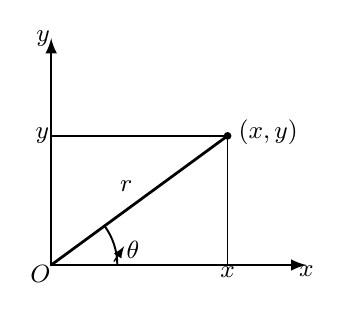
\begin{tikzpicture}[x=0.80cm, y=0.80cm, >=latex, line cap=round, line join=round]
  \draw[line width=0.9pt, ->] (0, 0) -- (4.05, 0) node[below=-1pt, inner sep=1pt] {\small $x$};
  \draw[line width=0.9pt, ->] (0, 0) -- (0, 3.60) node[left=-1pt, inner sep=1pt] {\small $y$};
  \node[below left=-1pt, inner sep=1pt] at (0, 0) {\small $O$};
  % 投影辅助线
  \draw[line width=0.6pt] (0, 2.05) -- (2.80, 2.05);
  \draw[line width=0.6pt] (2.80, 0) -- (2.80, 2.05);
  % 半径 r
  \draw[line width=1.0pt] (0, 0) -- (2.80, 2.05);
  \node[above left=-1pt, inner sep=1.5pt] at (1.32, 1.14) {\small $r$};
  % 夹角 theta
  \draw[line width=0.7pt] (1.05, 0) arc[start angle=0, end angle=36.2, radius=1.05];
  \draw[->, line width=0.5pt] (1.00, 0.06) -- (1.16, 0.30);
  \node[inner sep=1pt] at (1.30, 0.24) {\small $\theta$};
  % 端点
  \fill (2.80, 2.05) circle (1.4pt);
  \node[anchor=west, inner sep=1.5pt] at (2.90, 2.10) {\small $(x,y)$};
  \node[left=-1pt, inner sep=1.5pt] at (0, 2.05) {\small $y$};
  \node[below=-1pt, inner sep=1.5pt] at (2.80, 0) {\small $x$};
\end{tikzpicture}
\caption{}\label{fig:8.4.2}
\end{figure}

因此，$f$ 为局部 $C^{\infty}$ 微分同胚。但由 $f(1,0) = f(1,2\pi)$ 知 $f$ 非单射，从而整体的 $f^{-1}$ 不存在，$f$ 不为整体 $C^{\infty}$ 微分同胚。

再求 $r$，$\theta$ 关于 $x$，$y$ 的偏导数 $\dfrac{\partial r}{\partial x}$，$\dfrac{\partial r}{\partial y}$，$\dfrac{\partial\theta}{\partial x}$，$\dfrac{\partial\theta}{\partial y}$.
\end{example}

\begin{proof}[解法 1]
\begin{align*}
  \boldsymbol{J}f^{-1}(x,y) &= \bigl[\boldsymbol{J}f(\boldsymbol{r},\boldsymbol{\theta})\bigr]^{-1} \\
  &= \begin{pmatrix} \dfrac{\partial r}{\partial x} & \dfrac{\partial r}{\partial y} \\[6pt] \dfrac{\partial\theta}{\partial x} & \dfrac{\partial\theta}{\partial y} \end{pmatrix} = \begin{pmatrix} \dfrac{\partial x}{\partial r} & \dfrac{\partial x}{\partial\theta} \\[6pt] \dfrac{\partial y}{\partial r} & \dfrac{\partial y}{\partial\theta} \end{pmatrix}^{-1} = \begin{pmatrix} \cos\theta & -r\sin\theta \\ \sin\theta & r\cos\theta \end{pmatrix}^{-1} \\
  &= \frac{1}{r}\begin{pmatrix} r\cos\theta & r\sin\theta \\ -\sin\theta & \cos\theta \end{pmatrix} = \begin{pmatrix} \dfrac{x}{\sqrt{x^{2}+y^{2}}} & \dfrac{y}{\sqrt{x^{2}+y^{2}}} \\[8pt] -\dfrac{y}{x^{2}+y^{2}} & \dfrac{x}{x^{2}+y^{2}} \end{pmatrix}.
\end{align*}
\end{proof}

\begin{proof}[解法 2]
$r = \sqrt{x^{2}+y^{2}}$，$\theta = \arctan\dfrac{y}{x}$，因此
\[
  \frac{\partial r}{\partial x} = \frac{x}{\sqrt{x^{2}+y^{2}}},\quad \frac{\partial r}{\partial y} = \frac{y}{\sqrt{x^{2}+y^{2}}},
\]
\[
  \frac{\partial\theta}{\partial x} = \frac{-\dfrac{y}{x^{2}}}{1 + \left(\dfrac{y}{x}\right)^{2}} = -\frac{y}{x^{2}+y^{2}},\quad \frac{\partial\theta}{\partial y} = \frac{\dfrac{1}{x}}{1 + \left(\dfrac{y}{x}\right)^{2}} = \frac{x}{x^{2}+y^{2}}.
\]
\end{proof}

\begin{example}\label{ex:8.4.13}
设 $f: (0,+\infty) \times (0,\pi) \times (-\infty,+\infty) \to \mathbb{R}^{3}$，
\[
  (r,\theta,\varphi) \mapsto (x,y,z) = f(r,\theta,\varphi) = (r\sin\theta\cos\varphi,r\sin\theta\sin\varphi,r\cos\theta)
\]
为球坐标变换公式(图 8.4.3)，则
\begin{align*}
  \det \boldsymbol{J}f(\boldsymbol{r},\boldsymbol{\theta},\boldsymbol{\varphi}) &= \frac{\partial(x,y,z)}{\partial(r,\theta,\varphi)} = \begin{vmatrix} \dfrac{\partial x}{\partial r} & \dfrac{\partial x}{\partial\theta} & \dfrac{\partial x}{\partial\varphi} \\[6pt] \dfrac{\partial y}{\partial r} & \dfrac{\partial y}{\partial\theta} & \dfrac{\partial y}{\partial\varphi} \\[6pt] \dfrac{\partial z}{\partial r} & \dfrac{\partial z}{\partial\theta} & \dfrac{\partial z}{\partial\varphi} \end{vmatrix} \\
  &= \begin{vmatrix} \sin\theta\cos\varphi & r\cos\theta\cos\varphi & -r\sin\theta\sin\varphi \\ \sin\theta\sin\varphi & r\cos\theta\sin\varphi & r\sin\theta\cos\varphi \\ \cos\theta & -r\sin\theta & 0 \end{vmatrix} = r^{2}\sin\theta \neq 0.
\end{align*}

\begin{figure}[htbp]
\centering
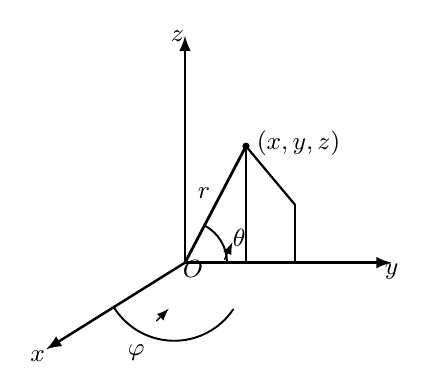
\begin{tikzpicture}[x=0.86cm, y=0.86cm, >=latex, line cap=round, line join=round]
  % 三轴
  \draw[line width=0.9pt, ->] (0, 0) -- (3.05, 0) node[below=-1pt, inner sep=1pt] {\small $y$};
  \draw[line width=0.9pt, ->] (0, 0) -- (0, 3.35) node[left=-1pt, inner sep=1pt] {\small $z$};
  \draw[line width=0.9pt, ->] (0, 0) -- (-2.05, -1.28) node[below left=-1pt, inner sep=1pt] {\small $x$};
  \node[below right=-2pt, inner sep=1pt] at (0, 0) {\small $O$};
  % 竖直投影三角形(母线)
  \draw[line width=0.8pt] (0.90, 0) -- (0.90, 1.72);
  \draw[line width=0.8pt] (0.90, 1.72) -- (1.62, 0.86);
  \draw[line width=0.8pt] (1.62, 0.86) -- (1.62, 0);
  % 半径 r
  \draw[line width=1.0pt] (0, 0) -- (0.90, 1.72);
  \node[above left=-1pt, inner sep=1.5pt] at (0.40, 0.92) {\small $r$};
  % theta 角
  \draw[line width=0.7pt] (0.62, 0) arc[start angle=0, end angle=62.4, radius=0.62];
  \draw[->, line width=0.5pt] (0.585, 0.05) -- (0.70, 0.30);
  \node[inner sep=1pt] at (0.80, 0.36) {\small $\theta$};
  % phi 角
  \draw[line width=0.7pt] (-1.05, -0.66) arc[start angle=212, end angle=326, radius=1.05];
  \draw[->, line width=0.5pt] (-0.42, -0.86) -- (-0.24, -0.68);
  \node[below=-1pt, inner sep=1pt] at (-0.72, -1.20) {\small $\varphi$};
  % 点 (x,y,z)
  \fill (0.90, 1.72) circle (1.3pt);
  \node[anchor=west, inner sep=1.5pt] at (0.99, 1.76) {\small $(x,y,z)$};
\end{tikzpicture}
\caption{}\label{fig:8.4.3}
\end{figure}

因此，$f$ 为局部 $C^{\infty}$ 微分同胚。但由 $f\left(1,\dfrac{\pi}{2},0\right) = f\left(1,\dfrac{\pi}{2},2\pi\right)$ 知，$f$ 非单射，从而整体的 $f^{-1}$ 不存在，$f$ 不为整体的 $C^{\infty}$ 微分同胚。
\end{example}

\begin{proof}[解法 1]
\begin{align*}
  \boldsymbol{J}f^{-1}(x,y,z) &= \bigl[\boldsymbol{J}f(\boldsymbol{r},\boldsymbol{\theta},\boldsymbol{\varphi})\bigr]^{-1} \\
  &= \begin{pmatrix} \dfrac{\partial r}{\partial x} & \dfrac{\partial r}{\partial y} & \dfrac{\partial r}{\partial z} \\[6pt] \dfrac{\partial\theta}{\partial x} & \dfrac{\partial\theta}{\partial y} & \dfrac{\partial\theta}{\partial z} \\[6pt] \dfrac{\partial\varphi}{\partial x} & \dfrac{\partial\varphi}{\partial y} & \dfrac{\partial\varphi}{\partial z} \end{pmatrix} \\
  &= \begin{pmatrix} \dfrac{\partial x}{\partial r} & \dfrac{\partial x}{\partial\theta} & \dfrac{\partial x}{\partial\varphi} \\[6pt] \dfrac{\partial y}{\partial r} & \dfrac{\partial y}{\partial\theta} & \dfrac{\partial y}{\partial\varphi} \\[6pt] \dfrac{\partial z}{\partial r} & \dfrac{\partial z}{\partial\theta} & \dfrac{\partial z}{\partial\varphi} \end{pmatrix}^{-1} \\
  &= \begin{pmatrix} \sin\theta\cos\varphi & r\cos\theta\cos\varphi & -r\sin\theta\sin\varphi \\ \sin\theta\sin\varphi & r\cos\theta\sin\varphi & r\sin\theta\cos\varphi \\ \cos\theta & -r\sin\theta & 0 \end{pmatrix}^{-1} \\
  &= \frac{1}{r^{2}\sin\theta}\begin{pmatrix} r^{2}\sin^{2}\theta\cos\varphi & r^{2}\sin^{2}\theta\sin\varphi & r^{2}\sin\theta\cos\theta \\ r\sin\theta\cos\theta\cos\varphi & r\sin\theta\cos\theta\sin\varphi & -r\sin^{2}\theta \\ -r\sin\varphi & r\cos\varphi & 0 \end{pmatrix} \\
  &= \begin{pmatrix} \sin\theta\cos\varphi & \sin\theta\sin\varphi & \cos\theta \\[4pt] \dfrac{\cos\theta\cos\varphi}{r} & \dfrac{\cos\theta\sin\varphi}{r} & -\dfrac{\sin\theta}{r} \\[8pt] -\dfrac{\sin\varphi}{r\sin\theta} & \dfrac{\cos\varphi}{r\sin\theta} & 0 \end{pmatrix} \\
  &= \begin{pmatrix} \dfrac{x}{r} & \dfrac{y}{r} & \dfrac{z}{r} \\[8pt] \dfrac{xz}{r^{2}\sqrt{x^{2}+y^{2}}} & \dfrac{yz}{r^{2}\sqrt{x^{2}+y^{2}}} & -\dfrac{\sqrt{x^{2}+y^{2}}}{r^{2}} \\[8pt] -\dfrac{y}{x^{2}+y^{2}} & \dfrac{x}{x^{2}+y^{2}} & 0 \end{pmatrix},
\end{align*}
其中 $x^{2}+y^{2} = r^{2}\sin^{2}\theta \neq 0$，$r = \sqrt{x^{2}+y^{2}+z^{2}} \neq 0$，
\[
  r = \sqrt{x^{2}+y^{2}+z^{2}},\quad \theta = \arccos\frac{z}{\sqrt{x^{2}+y^{2}+z^{2}}},\quad \varphi = \arcsin\frac{y}{\sqrt{x^{2}+y^{2}}}.
\]
通过简单计算，分别求出 $r$，$\theta$，$\varphi$ 对于 $x$，$y$，$z$ 的偏导数可以验证与上述结果完全一致.
\end{proof}

\begin{example}\label{ex:8.4.14}
设 $U \subset \mathbb{R}^{4}$ 为开集，$F$，$G: U \to \mathbb{R}^{1}$ 为 4 元函数。如果 $\boldsymbol{H} = (F,G)^{\mathrm{T}}$ 在点 $(z_{0},w_{0}) \in U$ (其中 $z_{0} = (x_{0},y_{0})$，$w_{0} = (u_{0},v_{0})$) 的某开邻域内满足隐射定理 8.4.2 的条件且 $\det \boldsymbol{J}_{w}H(z_{0},w_{0}) \neq 0$，则方程组 $\boldsymbol{H}(x,y,u,v) = \boldsymbol{0}$ 在点 $z_{0}$ 的某开邻域内能确定一个 $C^{k}$ 隐映 $w = f(z)$.
\end{example}

\begin{proof}[解法 1]
由定理 8.4.2 中的 (4) 求得
\[
  \boldsymbol{J}f(\boldsymbol{z}) = -\bigl[\boldsymbol{J}_{w}\boldsymbol{H}(\boldsymbol{z},\boldsymbol{w})\bigr]^{-1}\boldsymbol{J}_{z}\boldsymbol{H}(\boldsymbol{z},\boldsymbol{w}),
\]
即
\[
  \begin{pmatrix} \dfrac{\partial u}{\partial x} & \dfrac{\partial u}{\partial y} \\[6pt] \dfrac{\partial v}{\partial x} & \dfrac{\partial v}{\partial y} \end{pmatrix} = -\begin{pmatrix} \dfrac{\partial F}{\partial u} & \dfrac{\partial F}{\partial v} \\[6pt] \dfrac{\partial G}{\partial u} & \dfrac{\partial G}{\partial v} \end{pmatrix}^{-1}\begin{pmatrix} \dfrac{\partial F}{\partial x} & \dfrac{\partial F}{\partial y} \\[6pt] \dfrac{\partial G}{\partial x} & \dfrac{\partial G}{\partial y} \end{pmatrix}
\]
\begin{align*}
  &= -\frac{-1}{J}\begin{pmatrix} \dfrac{\partial G}{\partial v} & -\dfrac{\partial F}{\partial v} \\[6pt] -\dfrac{\partial G}{\partial u} & \dfrac{\partial F}{\partial u} \end{pmatrix}\begin{pmatrix} \dfrac{\partial F}{\partial x} & \dfrac{\partial F}{\partial y} \\[6pt] \dfrac{\partial G}{\partial x} & \dfrac{\partial G}{\partial y} \end{pmatrix} \\
  &= -\frac{1}{J}\begin{pmatrix} \dfrac{\partial(F,G)}{\partial(x,v)} & \dfrac{\partial(F,G)}{\partial(y,v)} \\[6pt] \dfrac{\partial(F,G)}{\partial(u,x)} & \dfrac{\partial(F,G)}{\partial(u,y)} \end{pmatrix},
\end{align*}
其中 $J = \dfrac{\partial(F,G)}{\partial(u,v)}$.
\end{proof}

\begin{proof}[解法 2]
设 $u = f(x,y)$，$v = g(x,y)$ 为由方程组
\[
  \left\{\begin{aligned}
    F(x,y,u,v) &= 0, \\
    G(x,y,u,v) &= 0
  \end{aligned}\right.
\]
所确定的隐函数，即
\[
  \left\{\begin{aligned}
    F(x,y,f(x,y),g(x,y)) &\equiv 0, \\
    G(x,y,f(x,y),g(x,y)) &\equiv 0.
  \end{aligned}\right.
\]
对上述方程组关于 $x$，$y$ 分别求偏导数得到
\begin{align*}
  &\left\{\begin{aligned}
    F_{x}^{\prime} + F_{u}^{\prime}u_{x}^{\prime} + F_{v}^{\prime}v_{x}^{\prime} &= 0, \\
    G_{x}^{\prime} + G_{u}^{\prime}u_{x}^{\prime} + G_{v}^{\prime}v_{x}^{\prime} &= 0,
  \end{aligned}\right. \\
  &\left\{\begin{aligned}
    F_{y}^{\prime} + F_{u}^{\prime}u_{y}^{\prime} + F_{v}^{\prime}v_{y}^{\prime} &= 0, \\
    G_{y}^{\prime} + G_{u}^{\prime}u_{y}^{\prime} + G_{v}^{\prime}v_{y}^{\prime} &= 0.
  \end{aligned}\right.
\end{align*}
因为
\[
  J = \frac{\partial(F,G)}{\partial(u,v)} = \begin{vmatrix} F_{u}^{\prime} & F_{v}^{\prime} \\ G_{u}^{\prime} & G_{v}^{\prime} \end{vmatrix} \neq 0,
\]
故从两个方程组分别解得
\[
  \frac{\partial u}{\partial x} = u_{x}^{\prime} = -\frac{1}{J}\frac{\partial(F,G)}{\partial(x,v)},\quad \frac{\partial u}{\partial y} = u_{y}^{\prime} = -\frac{1}{J}\frac{\partial(F,G)}{\partial(y,v)},
\]
\[
  \frac{\partial v}{\partial x} = v_{x}^{\prime} = -\frac{1}{J}\frac{\partial(F,G)}{\partial(u,x)},\quad \frac{\partial v}{\partial y} = v_{y}^{\prime} = -\frac{1}{J}\frac{\partial(F,G)}{\partial(u,y)}.
\]
\end{proof}

\begin{exblock}{练习题 8.4}
\item 下列方程确定隐函数 $y = y(x)$，计算 $\dfrac{\mathrm{d}y}{\mathrm{d}x}$;
\begin{enumerate}
  \item[(1)] $x^{2} + 2xy - y^{2} = a^{2}$;
  \item[(2)] $xy - \ln y = 0$，在点 $(0,1)$ 处;
  \item[(3)] $y - \varepsilon \sin y = x$，常数 $\varepsilon \in (0,1)$;
  \item[(4)] $x^{y} = y^{x}$
\end{enumerate}

\item 下列方程确定隐函数 $z = z(x,y)$，计算 $\dfrac{\partial z}{\partial x}$ 与 $\dfrac{\partial z}{\partial y}$.
\begin{enumerate}
  \item[(1)] $e^{x} - xyz = 0$;
  \item[(2)] $\dfrac{x}{z} = \ln\dfrac{z}{y}$;
  \item[(3)] $x + y + z = e^{-(x+y+z)}$，并对计算的结果作出解释;
  \item[(4)] $z^{2}y - xz^{3} - 1 = 0$，在点 $(1,2,1)$ 处.
\end{enumerate}

\item 设 $u = f(x,y,z,t)$，$g(y,z,t) = 0$，$h(z,t) = 0$，$f$，$g$ 与 $h$ 都一阶连续可导，计算 $\dfrac{\partial u}{\partial x}$ 与 $\dfrac{\partial u}{\partial y}$，并给出相应可计算的条件.

\item 设 $F(x-y,y-z,z-x) = 0$，$F$ 有一阶连续偏导数，计算 $\dfrac{\partial z}{\partial x}$ 与 $\dfrac{\partial z}{\partial y}$，并给出相应可计算的条件.

\item 设 $F(x+y+z,x^{2}+y^{2}+z^{2}) = 0$，$F$ 有一阶连续偏导数，计算 $\dfrac{\partial z}{\partial x}$ 与 $\dfrac{\partial z}{\partial y}$，并给出相应可计算的条件.

\item 二元函数 $F$ 在 $\mathbb{R}^{2}$ 上二次连续可导. 已知曲线 $F(x,y) = 0$ 呈“8”字形. 问方程组
\[
  \begin{cases}
    \dfrac{\partial F}{\partial x}(x,y) = 0, \\[4pt]
    \dfrac{\partial F}{\partial y}(x,y) = 0
  \end{cases}
\]
在 $\mathbb{R}^{2}$ 中至少有几组解?

\item 从方程组
\[
  \left\{\begin{aligned}
    x^{2} + y^{2} + z^{2} &= 1, \\
    x + y + z &= 0
  \end{aligned}\right.
\]
中，计算 $\dfrac{\mathrm{d}y}{\mathrm{d}x}$ 与 $\dfrac{\mathrm{d}z}{\mathrm{d}x}$，并作出几何解释.

\item 从方程组
\[
  \left\{\begin{aligned}
    x^{2} + y^{2} - z &= 0, \\
    x^{2} + 2y^{2} + 3z^{2} &= 20
  \end{aligned}\right.
\]
中，计算 $\dfrac{\mathrm{d}y}{\mathrm{d}x}$ 与 $\dfrac{\mathrm{d}z}{\mathrm{d}x}$，并作出几何解释.

\item 从下列方程中，计算 Jacobi 矩阵
\[
  \begin{pmatrix} \dfrac{\partial x}{\partial u} & \dfrac{\partial x}{\partial v} \\[6pt] \dfrac{\partial y}{\partial u} & \dfrac{\partial y}{\partial v} \end{pmatrix}.
\]
\begin{enumerate}
  \item[(1)] $xu - yv = 0$，$yu + xv = 1$;
  \item[(2)] $x + y = u + v$，$\dfrac{x}{y} = \dfrac{\sin u}{\sin v}$.
\end{enumerate}

\item 设
\[
  \left\{\begin{aligned}
    u^{2} - v\cos(xy) + w^{2} &= 0, \\
    u^{2} + v^{2} - \sin(xy) + 2w^{2} &= 2, \\
    uv - \sin x \cos y + w &= 0,
  \end{aligned}\right.
\]
试在 $(x,y) = \left(\dfrac{\pi}{2},0\right)$，$(u,v,w) = (1,1,0)$ 处计算 Jacobi 矩阵
\[
  \begin{pmatrix} \dfrac{\partial u}{\partial x} & \dfrac{\partial u}{\partial y} \\[6pt] \dfrac{\partial v}{\partial x} & \dfrac{\partial v}{\partial y} \\[6pt] \dfrac{\partial w}{\partial x} & \dfrac{\partial w}{\partial y} \end{pmatrix}.
\]

\item 从方程组
\[
  \left\{\begin{aligned}
    x &= t + \dfrac{1}{t}, \\
    y &= t^{2} + \dfrac{1}{t^{2}}, \\
    z &= t^{3} + \dfrac{1}{t^{3}}
  \end{aligned}\right.
\]
中，计算 $\dfrac{\mathrm{d}y}{\mathrm{d}x}$ 与 $\dfrac{\mathrm{d}z}{\mathrm{d}x}$.

\item 设 $U \subset \mathbb{R}^{n}$，$f: U \to \mathbb{R}^{n}$. 如果 $f$ 将开集映为开集，则称 $f$ 为一个开映射。问: 下列映射是否为开映射? 并说明理由。
\begin{enumerate}
  \item[(1)] $f(x,y) = \left(x^{2},\dfrac{y}{x}\right)$;
  \item[(2)] $f(x,y) = \left(\mathrm{e}^{x}\cos y,\mathrm{e}^{x}\sin y\right)$;
  \item[(3)] $f(x,y) = (x,x^{2})$
\end{enumerate}
进而，对 (1) 与 (2) 中的 $f$，计算 $\boldsymbol{J}f^{-1}$

\item 求由下列方程所确定的隐函数的偏导数:
\begin{enumerate}
  \item[(1)] $x + y + z = \mathrm{e}^{-(x+y+z)}$，求 $z$ 对 $x$，$y$ 的一阶与二阶偏导数;
  \item[(2)] $F(x,x+y,x+y+z) = 0$，$F$ 为 $C^{2}$ 函数，求 $\dfrac{\partial z}{\partial x}$，$\dfrac{\partial z}{\partial y}$，$\dfrac{\partial^{2} z}{\partial x^{2}}$.
\end{enumerate}

\item 设 $f$ 为一元函数，试问: $f$ 应满足什么条件，方程 $2f(xy) = f(x) + f(y)$ 在点 $(1,1)$ 的开邻域内能确定出惟一的 $y$ 为 $x$ 的函数?

\item 设 $F(x,y)$ 为 $C^{2}$ 函数，$F_{y}^{\prime} \neq 0$，证明: 由 $F(x,y) = 0$ 所确定的隐函数 $y = f(x)$ 有
\[
  \left(F_{y}^{\prime}\right)^{3} y'' = \begin{vmatrix} F_{xx}^{\prime\prime} & F_{xy}^{\prime\prime} & F_{x}^{\prime} \\ F_{xy}^{\prime\prime} & F_{yy}^{\prime\prime} & F_{y}^{\prime} \\ F_{x}^{\prime} & F_{y}^{\prime} & 0 \end{vmatrix}.
\]

\item 求由下列方程所确定的隐函数的极值:
\begin{enumerate}
  \item[(1)] $x^{2} + 2xy + 2y^{2} = 1$
  \item[(2)] $(x^{2}+y^{2}) = a^{2}(x^{2}-y^{2})$ $(a > 0)$
\end{enumerate}

\item 设 $f$，$g$，$h$ 可微，
\[
  \begin{cases}
    x = f(u,v,w), \\
    y = g(u,v,w), \\
    z = h(u,v,w),
  \end{cases}
\]
求 $\dfrac{\partial u}{\partial x}$，$\dfrac{\partial u}{\partial y}$，$\dfrac{\partial u}{\partial z}$，并给出可计算的条件.

\item 设 $f$，$g$ 为可微函数，求下列方程所确定的隐函数 $u = u(x,y)$ 的偏导数 $\dfrac{\partial u}{\partial x}$，$\dfrac{\partial u}{\partial y}$
\begin{enumerate}
  \item[(1)] $x^{2} + u^{2} = f(x,u) + g(x,y,u)$;
  \item[(2)] $u = f(x + u,yu)$.
\end{enumerate}
进而给出可计算的条件.

\item 设 $y = f(x)$ 为 $C^{1}$ 函数，$x = \varphi(u,v)$，$y = \psi(u,v)$ 为 $C^{2}$ 函数，则由方程 $\psi(u,v) = f(\varphi(u,v))$ 可以确定函数 $v = v(u)$. 试用 $u$，$v$，$\dfrac{\mathrm{d}v}{\mathrm{d}u}$，$\dfrac{\mathrm{d}^{2}v}{\mathrm{d}u^{2}}$ 表示 $\dfrac{\mathrm{d}y}{\mathrm{d}x}$，$\dfrac{\mathrm{d}^{2}y}{\mathrm{d}x^{2}}$; 并给出可计算的条件.
\end{exblock}

\begin{exblock}{思考题 8.4}
\item 设 $(x_{0},y_{0},z_{0},u_{0})$ 满足方程组
\[
  \left\{\begin{aligned}
    f(x) + f(y) + f(z) &= F(u), \\
    g(x) + g(y) + g(z) &= G(u), \\
    h(x) + h(y) + h(z) &= H(u),
  \end{aligned}\right.
\]
这里所有的函数假定有连续的导数.

(1) 说出一个能在该点开邻域内确定 $x$，$y$，$z$ 为 $u$ 的函数的充分条件;

(2) 在 $f(x) = x$，$g(x) = x^{2}$，$h(x) = x^{3}$ 的情形下，上述条件相当于什么?

\item 据理说明: 在点 $(0,1)$ 近旁是否存在 $C^{\infty}$ 的 $f(x,y)$ 与 $g(x,y)$ 满足:
\[
  f(0,1) = 1,\quad g(0,1) = -1,
\]
且
\[
  \left\{\begin{aligned}
    [f(x,y)]^{3} + x g(x,y) - y &= 0, \\
    [g(x,y)]^{3} + y f(x,y) - x &= 0.
  \end{aligned}\right.
\]
\end{exblock}
